%2multibyte Version: 5.50.0.2960 CodePage: 65001
% !TeX root = ./Slides_Lez_15_Programmazione_Stocastica_II.tex
%******************
% Slides Lezione 15 - Programmazione lineare stocastica II
% Versione a due stadi: soluzione e valore dell'informazione
% Progetto MQF - Metodi Quantitativi per la Finanza
% Macro matematiche ufficiali del progetto MQF
% Coerenti con MQF_Notazione.tex
% Vocali accentate nella forma \`a, \`e, \'e, senza parentesi graffe
%******************
% Fallback utile per compilazione esterna se qualche titolo resta scritto come \QTR.
% Scientific WorkPlace usa \QTR internamente; in Beamer \QTR{frametitle}{Titolo}
% deve espandersi in \frametitle{Titolo}.

\documentclass[handout]{beamer}%
\usepackage{mathpazo}
%\usepackage{hyperref}
\usepackage{multimedia}
\usepackage{amsmath}
\usepackage{amsfonts}
\usepackage{amssymb}
\usepackage{graphicx}%
\setcounter{MaxMatrixCols}{30}
%TCIDATA{OutputFilter=latex2.dll}
%TCIDATA{Version=5.50.0.2960}
%TCIDATA{Codepage=65001}
%TCIDATA{CSTFile=beamer.cst}
%TCIDATA{<META NAME="GraphicsSave" CONTENT="32">}
%TCIDATA{<META NAME="SaveForMode" CONTENT="2">}
%TCIDATA{BibliographyScheme=Manual}
%TCIDATA{<META NAME="DocumentShell" CONTENT="Other Documents\SW\Slides - Beamer">}
%BeginMSIPreambleData
\providecommand{\U}[1]{\protect\rule{.1in}{.1in}}
%EndMSIPreambleData
\newenvironment{stepenumerate}{\begin{enumerate}[<+->]}{\end{enumerate}}
\newenvironment{stepitemize}{\begin{itemize}[<+->]}{\end{itemize} }
\newenvironment{stepenumeratewithalert}{\begin{enumerate}[<+-| alert@+>]}{\end{enumerate}}
\newenvironment{stepitemizewithalert}{\begin{itemize}[<+-| alert@+>]}{\end{itemize} }
\usetheme{Madrid}

\setbeamertemplate{footline}
{
  \leavevmode%
  \hbox{%
    \begin{beamercolorbox}[wd=.20\paperwidth,ht=2.25ex,dp=1ex,center]
      {author in head/foot}%
      \usebeamerfont{author in head/foot}\insertshortauthor
    \end{beamercolorbox}%
    \begin{beamercolorbox}[wd=.69\paperwidth,ht=2.25ex,dp=1ex,center]
      {title in head/foot}%
      \usebeamerfont{title in head/foot}\insertshorttitle
    \end{beamercolorbox}%
    \begin{beamercolorbox}[wd=.11\paperwidth,ht=2.25ex,dp=1ex,right]
      {date in head/foot}%
      \usebeamerfont{date in head/foot}%
      \insertshortdate{}\hspace*{2em}%
      \insertframenumber{} / \inserttotalframenumber\hspace*{2ex}
    \end{beamercolorbox}%
  }%
  \vskip0pt%
}


\providecommand{\R}{\mathbb{R}}
\providecommand{\N}{\mathbb{N}}
\providecommand{\E}{\mathbb{E}}
\providecommand{\Prob}{\mathbb{P}}
\providecommand{\Q}{\mathbb{Q}}
\providecommand{\F}{\mathcal{F}}
\providecommand{\B}{\mathcal{B}}
\providecommand{\G}{\mathcal{G}}
\providecommand{\Var}{\operatorname{Var}}
\providecommand{\Cov}{\operatorname{Cov}}
\providecommand{\VaR}{\operatorname{VaR}}
\providecommand{\CVaR}{\operatorname{CVaR}}
\providecommand{\argmin}{\operatorname*{arg\,min}}
\providecommand{\argmax}{\operatorname*{arg\,max}}
\providecommand{\EVPI}{\operatorname{EVPI}}
\providecommand{\VSS}{\operatorname{VSS}}
\providecommand{\QTR}[2]{\csname #1\endcsname{#2}}
%BeginMSIPreambleData
\ifx\pdfoutput\relax\let\pdfoutput=\undefined\fi
\newcount\msipdfoutput
\ifx\pdfoutput\undefined\else
\ifcase\pdfoutput\else
\msipdfoutput=1
\ifx\paperwidth\undefined\else
\ifdim\paperheight=0pt\relax\else\pdfpageheight\paperheight\fi
\ifdim\paperwidth=0pt\relax\else\pdfpagewidth\paperwidth\fi
\fi\fi\fi
%EndMSIPreambleData


\title[Lez. 15 - Programmazione lineare stocastica II]{Lezione 15 - Programmazione lineare stocastica II}
\subtitle{Metodi Quantitativi per la Finanza}
\author[P. Falbo, C. Pelizzari]{{\LARGE Paolo Falbo, Cristian Pelizzari}}
\institute[]{{\large Dipartimento di Economia e Management}}
\date[]{}
\titlegraphic{

\includegraphics[height=1.25cm]{../graphics/MQF_logo.png}\hspace{0.8cm}%

\includegraphics[height=1.25cm]{../graphics/logo-Unibs-esteso.png}
}

\begin{document}
\maketitle

%****************************************

\section{Apertura}

\subsection{Il programma a due stadi}%

%TCIMACRO{\TeXButton{BeginFrame}{\begin{frame}}}%
%BeginExpansion
\begin{frame}%
%EndExpansion

\QTR{frametitle}{Richiamo: il programma a due stadi}

%TCIMACRO{\TeXButton{Transparency}{\setbeamercovered{transparent=20}}}%
%BeginExpansion
\setbeamercovered{transparent=20}%
%EndExpansion

Nel Capitolo~14 la decisione iniziale $x$ viene assunta prima di conoscere lo
scenario; dopo l'osservazione dello scenario $s$ il piano si adatta con il
ricorso $y_s$.

{\small
\[
\max_{x\in\mathcal X_0}
\Big\{
c'x+\sum_{s\in\mathcal S}p_sQ_s(x)
\Big\},
\qquad
Q_s(x)
=
\max_{y_s\in\mathcal X_s}
\left\{
q_s'y_s:\;
T_sx+W_sy_s=h_s
\right\}.
\]
}

\begin{stepitemize}
\item $x$ \`e \textbf{unica} e comune a tutti gli scenari.

\item $y_s$ viene scelto dopo l'osservazione dello scenario e pu\`o quindi
dipendere da esso.

\item $Q_s(x)$ \`e il valore ottimo del problema di secondo stadio nello
scenario $s$.
\end{stepitemize}

\medskip

{\footnotesize Caso SVB-ALM: $x=(x_1,x_2,x_3,x_4)'$ \`e la composizione
iniziale dell'attivo; $y_s=(g_1^s,\ldots,g_4^s,u_1^s,u_2^s,u_3^s)'$ raccoglie
giacenze e funding alle diverse date.}

%TCIMACRO{\TeXButton{Transition: Box Out}{\transboxout}}%
%BeginExpansion
\transboxout%
%EndExpansion
%TCIMACRO{\TeXButton{EndFrame}{\end{frame}}}%
%BeginExpansion
\end{frame}%
%EndExpansion

%****************************************

\subsection{Le domande della lezione}%

%TCIMACRO{\TeXButton{BeginFrame}{\begin{frame}}}%
%BeginExpansion
\begin{frame}%
%EndExpansion

\QTR{frametitle}{Le domande della lezione}

%TCIMACRO{\TeXButton{Transparency}{\setbeamercovered{transparent=20}}}%
%BeginExpansion
\setbeamercovered{transparent=20}%
%EndExpansion

La formulazione chiarisce la struttura di una decisione sotto incertezza, ma
lascia aperte alcune questioni che riguardano la sua soluzione.

\medskip

\begin{stepenumerate}
\item [1.] \textbf{Fattibilit\`a.} Fissata $x$ e osservato lo scenario $s$,
esiste una decisione di ricorso che soddisfa i vincoli?

\item [2.] \textbf{Dipendenza da $x$.} Come varia il valore del ricorso
$Q_s(x)$ al variare della decisione iniziale?

\item [3.] \textbf{Valore.} Quanto vale scegliere $x$ tenendo conto degli
scenari, anzich\'e dei soli valori medi? E quanto varrebbe conoscere il
futuro?
\end{stepenumerate}

\medskip

\begin{block}{Domanda guida}
{\small Quali propriet\`a deve possedere una decisione stocastica, come si
determina il compromesso tra scenari differenti e quanto vale disporre di una
migliore informazione sul futuro?}
\end{block}

%TCIMACRO{\TeXButton{Transition: Box Out}{\transboxout}}%
%BeginExpansion
\transboxout%
%EndExpansion
%TCIMACRO{\TeXButton{EndFrame}{\end{frame}}}%
%BeginExpansion
\end{frame}%
%EndExpansion

%****************************************

\subsection{Percorso della lezione}%

%TCIMACRO{\TeXButton{BeginFrame}{\begin{frame}}}%
%BeginExpansion
\begin{frame}%
%EndExpansion

\QTR{frametitle}{Percorso e obiettivi}

%TCIMACRO{\TeXButton{Transparency}{\setbeamercovered{transparent=20}}}%
%BeginExpansion
\setbeamercovered{transparent=20}%
%EndExpansion

In questa lezione, i temi del Capitolo 15 vengono approfonditi nel framework a due stadi, cos\`i da isolare le propriet\`a della soluzione senza introdurre anche la struttura multistadio.

\begin{stepenumerate}
\item [1.] \textbf{Fattibilit\`a del ricorso}: quando una decisione iniziale
lascia una correzione possibile in ogni scenario.

\item [2.] \textbf{Funzione di ricorso}: come il valore dell'adattamento
dipende da $x$.

\item [3.] \textbf{Scelta di $x$}: il compromesso fra redditivit\`a iniziale e
costo atteso del ricorso.

\item [4.] \textbf{Tre benchmark}: soluzione stocastica, wait-and-see, valori
medi; $\EVPI$ e $\VSS$.

\item [5.] \textbf{Forma estesa e scenari}: il programma lineare che il solver
ricever\`a nella Lezione~16.
\end{stepenumerate}

\medskip

Sei esercizi in aula accompagnano il percorso.

\medskip

\begin{center}
{\small \emph{Chiave di lettura: la programmazione stocastica cerca la migliore
decisione compatibile con l'informazione disponibile nel momento in cui essa
deve essere assunta.}}
\end{center}

%TCIMACRO{\TeXButton{Transition: Box Out}{\transboxout}}%
%BeginExpansion
\transboxout%
%EndExpansion
%TCIMACRO{\TeXButton{EndFrame}{\end{frame}}}%
%BeginExpansion
\end{frame}%
%EndExpansion

%****************************************

\section{Fattibilit\`a del ricorso}

\subsection{Il ricorso esiste}%

%TCIMACRO{\TeXButton{BeginFrame}{\begin{frame}}}%
%BeginExpansion
\begin{frame}%
%EndExpansion

\QTR{frametitle}{Il ricorso esiste?}

%TCIMACRO{\TeXButton{Transparency}{\setbeamercovered{transparent=20}}}%
%BeginExpansion
\setbeamercovered{transparent=20}%
%EndExpansion

Fissate la decisione iniziale $x$ e lo scenario $s$, il problema di secondo
stadio \`e

{\small
\[
Q_s(x)
=
\max_{y_s\in\mathcal X_s}
\left\{
q_s'y_s:\;
T_sx+W_sy_s=h_s
\right\}.
\]
}

Il valore $Q_s(x)$ \`e definito solo se l'insieme delle decisioni di ricorso
ammissibili non \`e vuoto.

\medskip

\begin{block}{Ricorso ammissibile}
{\small Fissati $x\in\mathcal X_0$ e $s\in\mathcal S$, il ricorso \`e
\emph{ammissibile} se esiste almeno una decisione $y_s\in\mathcal X_s$ tale che
$T_sx+W_sy_s=h_s$.}
\end{block}

\medskip

\begin{stepitemize}
\item La propriet\`a riguarda la singola coppia $(x,s)$: la stessa $x$ pu\`o
ammettere ricorso in uno scenario e non in un altro.

\item \textbf{Ammissibile non significa conveniente}: due decisioni con ricorso
ammissibile possono produrre valori di $Q_s(x)$ molto diversi.
\end{stepitemize}

%TCIMACRO{\TeXButton{Transition: Box Out}{\transboxout}}%
%BeginExpansion
\transboxout%
%EndExpansion
%TCIMACRO{\TeXButton{EndFrame}{\end{frame}}}%
%BeginExpansion
\end{frame}%
%EndExpansion

%****************************************

\subsection{Completo e relativamente completo}%

%TCIMACRO{\TeXButton{BeginFrame}{\begin{frame}}}%
%BeginExpansion
\begin{frame}%
%EndExpansion

\QTR{frametitle}{Ricorso completo e relativamente completo}

%TCIMACRO{\TeXButton{Transparency}{\setbeamercovered{transparent=20}}}%
%BeginExpansion
\setbeamercovered{transparent=20}%
%EndExpansion

\begin{block}{Ricorso completo}
{\small Il secondo stadio \`e ammissibile per \textbf{qualunque} termine noto
del sistema di ricorso.}
\end{block}

\begin{block}{Ricorso relativamente completo}
{\small Il secondo stadio \`e ammissibile per i termini noti \textbf{generati}
da $x\in\mathcal X_0$ e dagli scenari del modello.}
\end{block}

\medskip

\begin{stepitemize}
\item Il ricorso completo implica quello relativamente completo; il contrario
non vale in generale.

\item Restringendo l'insieme $\mathcal X_0$ si pu\`o ottenere ricorso
relativamente completo anche senza ricorso completo.

\item \textbf{Lettura ALM}: il funding ha limiti di capacit\`a. Non serve
compensare qualunque deficit immaginabile, ma i deficit generati dalle
decisioni ammissibili negli scenari del modello.
\end{stepitemize}

%TCIMACRO{\TeXButton{Transition: Box Out}{\transboxout}}%
%BeginExpansion
\transboxout%
%EndExpansion
%TCIMACRO{\TeXButton{EndFrame}{\end{frame}}}%
%BeginExpansion
\end{frame}%
%EndExpansion

%****************************************

\subsection{Un esempio con capacit\`a limitata}%

%TCIMACRO{\TeXButton{BeginFrame}{\begin{frame}}}%
%BeginExpansion
\begin{frame}%
%EndExpansion

\QTR{frametitle}{Esempio: funding con capacit\`a limitata}

%TCIMACRO{\TeXButton{Transparency}{\setbeamercovered{transparent=20}}}%
%BeginExpansion
\setbeamercovered{transparent=20}%
%EndExpansion

{\small Due classi di attivo, $A_0=10$; $x$ \`e l'investimento nella classe
pi\`u liquida, la composizione \`e $(x,\;10-x)'$ con $0\leq x\leq10$.
Fabbisogno $d=8$; dopo lo scenario: funding $0\leq u_s\leq\bar u_s$ e
giacenza $g_s\geq0$, con bilancio $a_s'(x,\;10-x)'+u_s=8+g_s$.}

{\small
\[
a_1'=(1,\;0.6),
\qquad
a_2'=(1,\;0.2),
\qquad
\bar u_1=1,
\qquad
\bar u_2=2.
\]
}

Il funding minimo necessario in ciascuno scenario \`e

{\small
\[
\begin{aligned}
u_1^{\min}(x)&=\max\{0,\;2-0.4x\}\leq1
&&\iff\quad x\geq2.5,\\
u_2^{\min}(x)&=\max\{0,\;6-0.8x\}\leq2
&&\iff\quad x\geq5.
\end{aligned}
\]
}

\begin{stepitemize}
\item $x=4$: $u_1^{\min}=0.4<1$, ma $u_2^{\min}=2.8>2$. Il ricorso \`e
ammissibile solo nello scenario ordinario.

\item $x=6$: $u_1^{\min}=0$ e $u_2^{\min}=1.2<2$. Il ricorso \`e ammissibile
in entrambi gli scenari.
\end{stepitemize}

%TCIMACRO{\TeXButton{Transition: Box Out}{\transboxout}}%
%BeginExpansion
\transboxout%
%EndExpansion
%TCIMACRO{\TeXButton{EndFrame}{\end{frame}}}%
%BeginExpansion
\end{frame}%
%EndExpansion

%****************************************

\subsection{Tre regioni}%

%TCIMACRO{\TeXButton{BeginFrame}{\begin{frame}}}%
%BeginExpansion
\begin{frame}%
%EndExpansion

\QTR{frametitle}{Tre regioni di ammissibilit\`a}

%TCIMACRO{\TeXButton{Transparency}{\setbeamercovered{transparent=20}}}%
%BeginExpansion
\setbeamercovered{transparent=20}%
%EndExpansion

\begin{center}
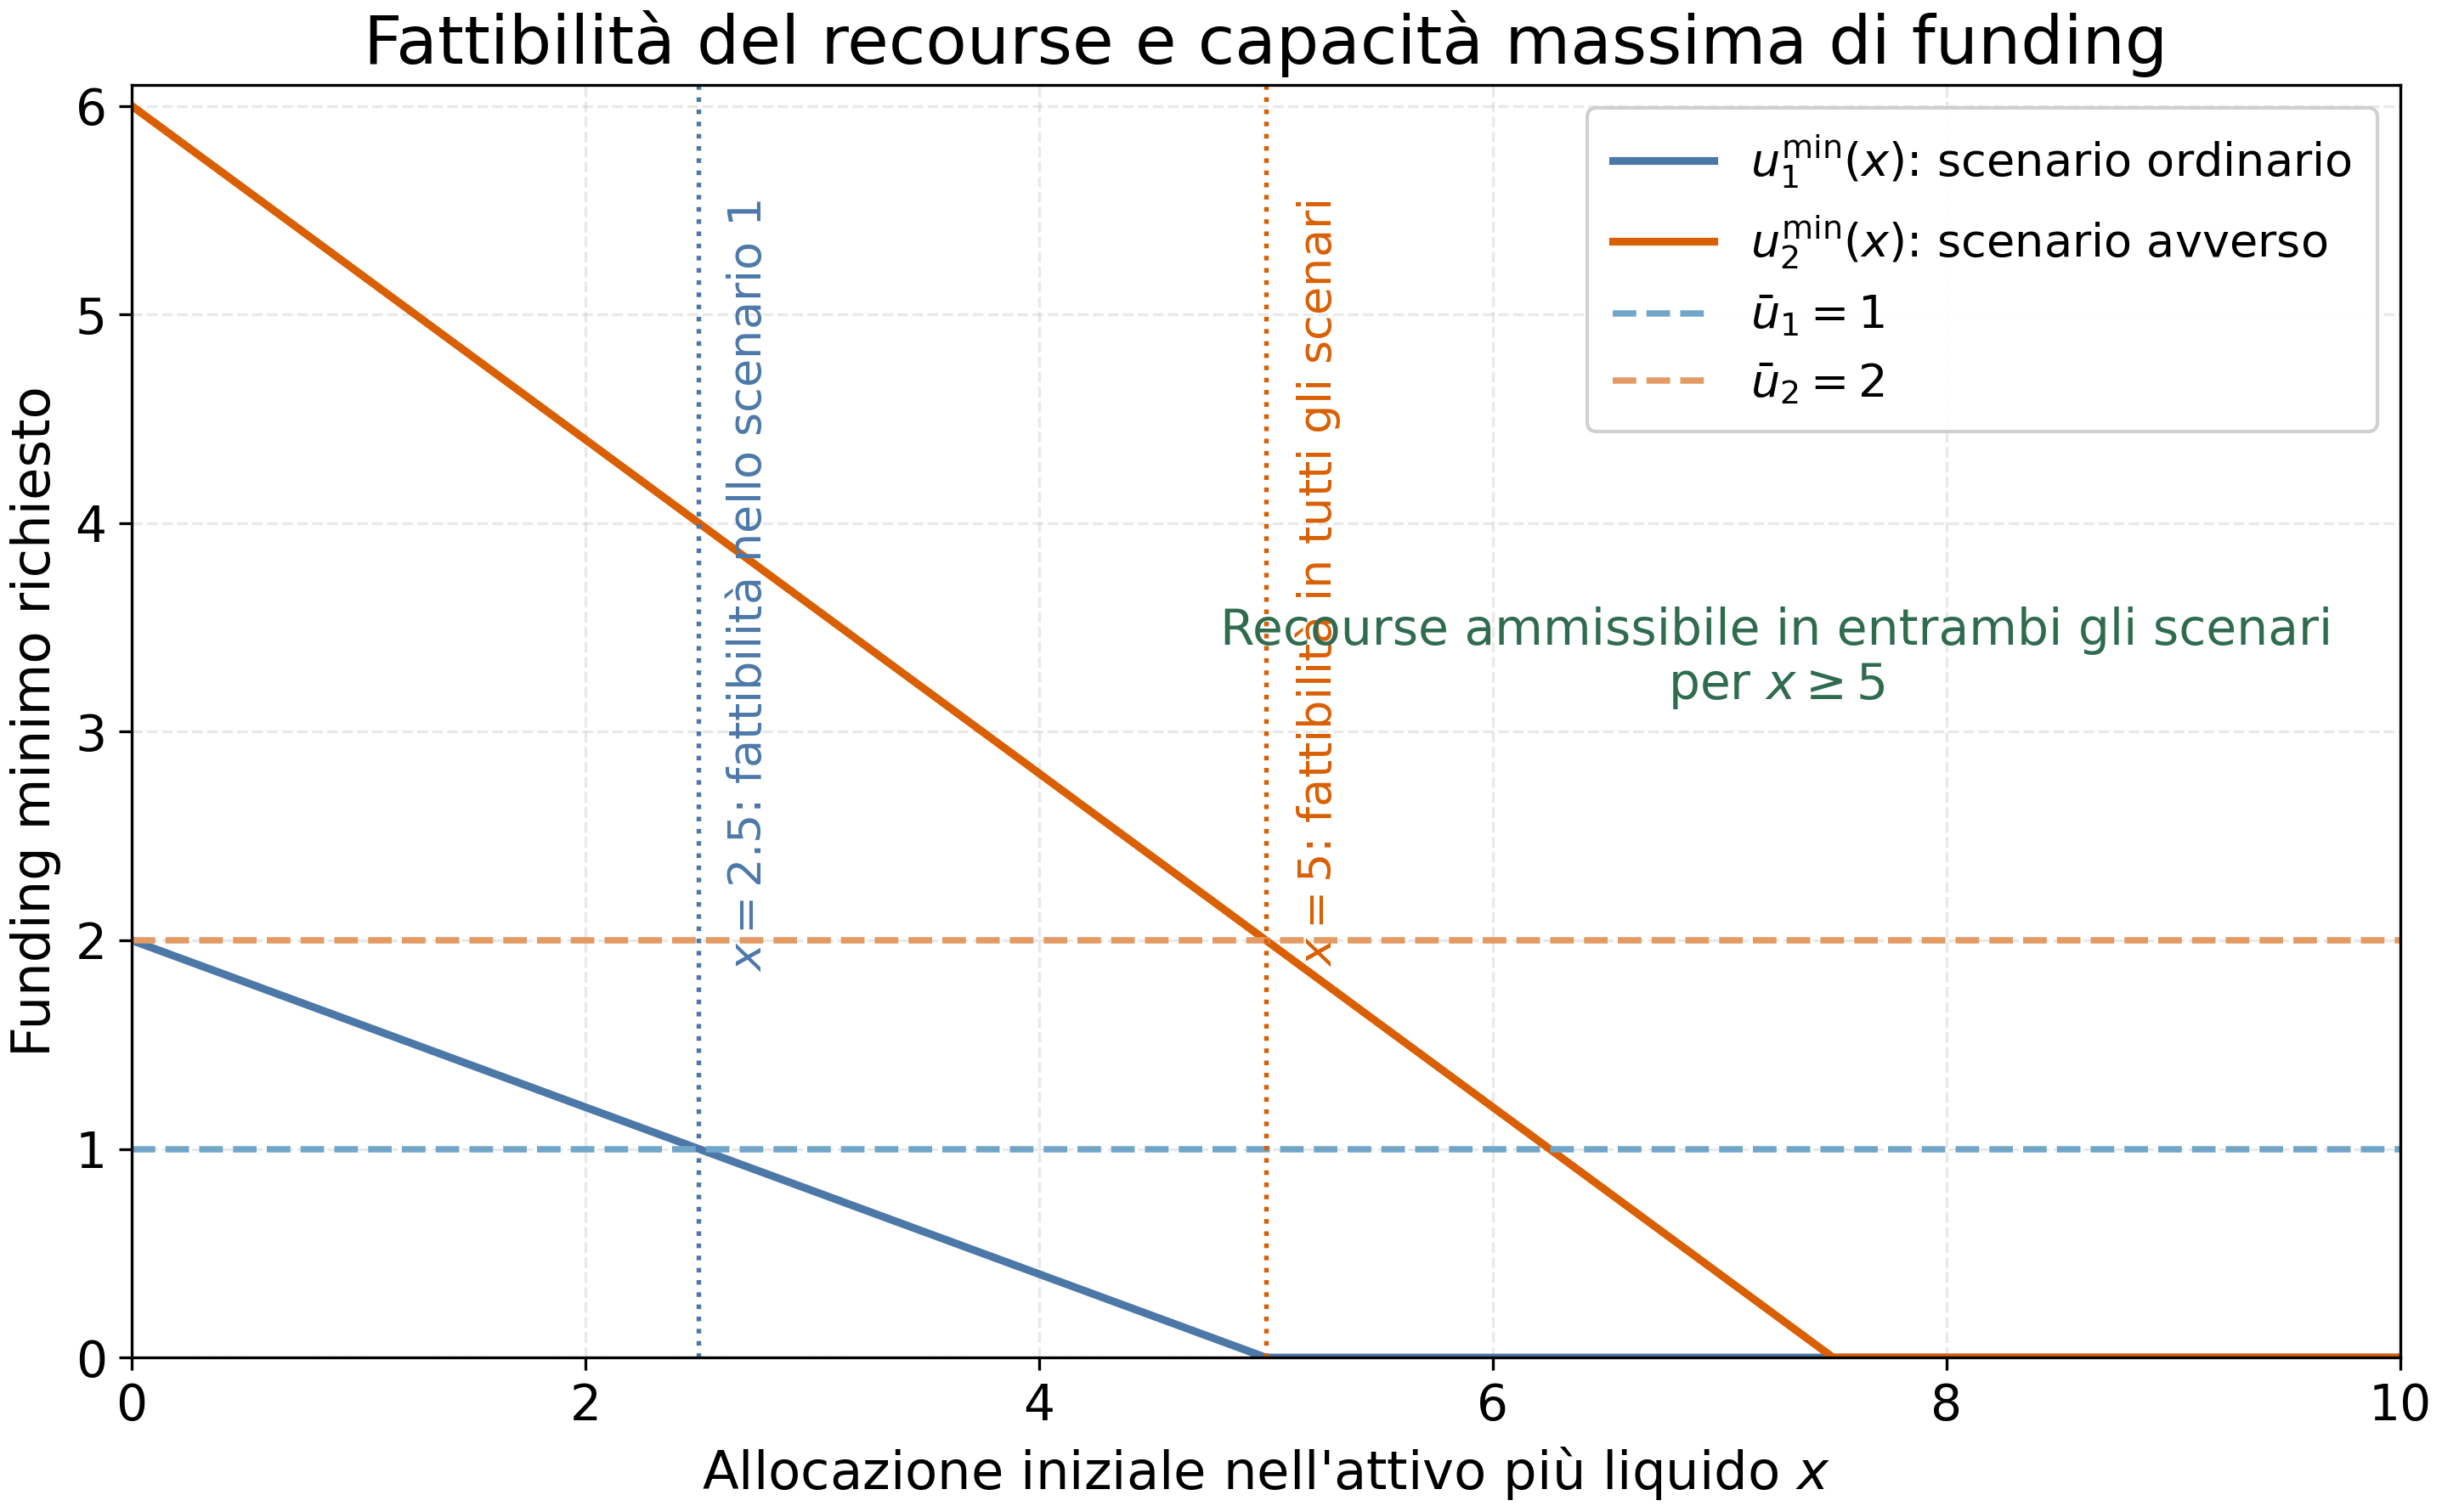
\includegraphics[width=0.56\textwidth]
{../graphics/Cap15_fattibilita_ricorso.png}
\end{center}

\vspace{-3mm}

{\small
\begin{stepitemize}
\item $0\leq x<2.5$: nessuno scenario; $\;2.5\leq x<5$: solo l'ordinario;
$\;x\geq5$: entrambi.

\item $\mathcal X_0=[0,10]$: niente ricorso relativamente completo ($x=4$).
$\mathcal X_0=[5,10]$: relativamente completo, ma non completo.

\item La fattibilit\`a \`e il \textbf{primo filtro}: solo dopo ha senso
studiare il valore economico del ricorso.
\end{stepitemize}
}

%TCIMACRO{\TeXButton{Transition: Box Out}{\transboxout}}%
%BeginExpansion
\transboxout%
%EndExpansion
%TCIMACRO{\TeXButton{EndFrame}{\end{frame}}}%
%BeginExpansion
\end{frame}%
%EndExpansion

%****************************************

\section{Esercizio in aula: limite alla capacit\`a di funding}

\subsection{La consegna}%

%TCIMACRO{\TeXButton{BeginFrame}{\begin{frame}}}%
%BeginExpansion
\begin{frame}%
%EndExpansion

\QTR{frametitle}{Esercizio: limite alla capacit\`a di funding}

%TCIMACRO{\TeXButton{Transparency}{\setbeamercovered{transparent=20}}}%
%BeginExpansion
\setbeamercovered{transparent=20}%
%EndExpansion

{\footnotesize (Capitolo~14, Esercizio proposto~4)}

\medskip

Si consideri la decisione di primo stadio e uno scenario avverso con

\[
x=
\begin{pmatrix}
3\\
7
\end{pmatrix},
\qquad
a'=(1,\;0.25),
\qquad
d=6.
\]

Il ricorso utilizza le variabili $g\geq0$ e $0\leq u\leq\bar u$, con vincolo
$a'x+u=d+g$.

\medskip

\begin{stepenumerate}
\item [1.] Determinare il funding minimo necessario per rendere ammissibile la
decisione assegnata.

\item [2.] Stabilire se il problema di secondo stadio \`e ammissibile per
$\bar u=2$.

\item [3.] Ripetere l'analisi per $\bar u=1$.

\item [4.] Spiegare come il limite alla capacit\`a di funding modifica il
significato della funzione di ricorso.
\end{stepenumerate}

%TCIMACRO{\TeXButton{Transition: Box Out}{\transboxout}}%
%BeginExpansion
\transboxout%
%EndExpansion
%TCIMACRO{\TeXButton{EndFrame}{\end{frame}}}%
%BeginExpansion
\end{frame}%
%EndExpansion

%****************************************

\subsection{La soluzione}%

%TCIMACRO{\TeXButton{BeginFrame}{\begin{frame}}}%
%BeginExpansion
\begin{frame}%
%EndExpansion

\QTR{frametitle}{Soluzione: il deficit e la capacit\`a}

%TCIMACRO{\TeXButton{Transparency}{\setbeamercovered{transparent=20}}}%
%BeginExpansion
\setbeamercovered{transparent=20}%
%EndExpansion

\begin{stepenumerate}
\item [1.] La liquidit\`a generata dalla decisione assegnata \`e
\[
a'x=3+0.25\cdot7=4.75<6
\qquad\Longrightarrow\qquad
u^{\min}=6-4.75=1.25.
\]

\item [2.] Con $\bar u=2\geq1.25$ il problema di secondo stadio \`e
ammissibile, per esempio con $u=1.25$ e $g=0$.

\item [3.] Con $\bar u=1<1.25$ nessuna coppia $(g,u)$ soddisfa il bilancio:
il problema di secondo stadio \textbf{non} \`e ammissibile.

\item [4.] La funzione di ricorso ha significato solo dove la capacit\`a di
funding copre il deficit: il limite restringe le decisioni iniziali per le
quali il ricorso esiste.
\end{stepenumerate}

\medskip

\begin{center}
{\small Prima di valutare $Q(x)$ occorre verificare che il secondo stadio
ammetta soluzioni.}
\end{center}

%TCIMACRO{\TeXButton{Transition: Box Out}{\transboxout}}%
%BeginExpansion
\transboxout%
%EndExpansion
%TCIMACRO{\TeXButton{EndFrame}{\end{frame}}}%
%BeginExpansion
\end{frame}%
%EndExpansion

%****************************************

\section{La funzione di ricorso}

\subsection{Dipendenza dalla decisione iniziale}%

%TCIMACRO{\TeXButton{BeginFrame}{\begin{frame}}}%
%BeginExpansion
\begin{frame}%
%EndExpansion

\QTR{frametitle}{La decisione iniziale cambia il problema futuro}

%TCIMACRO{\TeXButton{Transparency}{\setbeamercovered{transparent=20}}}%
%BeginExpansion
\setbeamercovered{transparent=20}%
%EndExpansion

Fissato lo scenario $s$, la decisione iniziale entra nel secondo stadio
attraverso il termine noto
\[
h_s-T_sx.
\]
Decisioni diverse $x'$ e $x''$ producono, in generale,
$Q_s(x')\neq Q_s(x'')$: la qualit\`a di $x$ dipende da $c'x$ \textbf{e} dal
suo effetto sul ricorso.

\medskip

\begin{block}{Proposizione}
{\small Se il problema di secondo stadio \`e ammissibile per i valori di $x$
considerati e possiede valore ottimo finito, $Q_s(x)$ \`e \textbf{concava e
lineare a tratti} rispetto a $x$ sul proprio dominio di fattibilit\`a.}
\end{block}

\medskip

\begin{stepitemize}
\item Il valore marginale di una variazione di $x$ \`e costante all'interno di
ciascun tratto lineare.

\item La pendenza cambia quando cambia la struttura della soluzione ottima di
secondo stadio.
\end{stepitemize}

%TCIMACRO{\TeXButton{Transition: Box Out}{\transboxout}}%
%BeginExpansion
\transboxout%
%EndExpansion
%TCIMACRO{\TeXButton{EndFrame}{\end{frame}}}%
%BeginExpansion
\end{frame}%
%EndExpansion

%****************************************

\subsection{Un esempio unidimensionale}%

%TCIMACRO{\TeXButton{BeginFrame}{\begin{frame}}}%
%BeginExpansion
\begin{frame}%
%EndExpansion

\QTR{frametitle}{Esempio: lo scenario avverso}

%TCIMACRO{\TeXButton{Transparency}{\setbeamercovered{transparent=20}}}%
%BeginExpansion
\setbeamercovered{transparent=20}%
%EndExpansion

{\small $A_0=10\,000$ milioni di euro, $x_1+x_2=10\,000$; $x_1$ \`e l'attivo
pi\`u liquido. Nello scenario avverso, con fabbisogno $d=6\,000$ e funding al
costo del $3\%$:}

{\small
\[
x_1+0.2x_2+u_2=6\,000+g_2,
\qquad
Q_2=-0.03\,u_2.
\]
}

{\small Sostituendo $x_2=10\,000-x_1$:}

{\small
\[
u_2^*(x_1)=\max\{0,\;4\,000-0.8x_1\},
\]
\[
Q_2(x_1)=
\begin{cases}
-120+0.024x_1, & 0\leq x_1\leq5\,000,\\[2pt]
0, & 5\,000\leq x_1\leq10\,000.
\end{cases}
\]
}

\begin{stepitemize}
\item Verifica: $x_1=2\,000$ $\Rightarrow$ $u_2^*=2\,400$, $C_2=72$,
$Q_2=-72$.

\item Il coefficiente $0.2$ \`e la quota dell'investimento disponibile alla
data del fabbisogno, \textbf{non} un rendimento.
\end{stepitemize}

%TCIMACRO{\TeXButton{Transition: Box Out}{\transboxout}}%
%BeginExpansion
\transboxout%
%EndExpansion
%TCIMACRO{\TeXButton{EndFrame}{\end{frame}}}%
%BeginExpansion
\end{frame}%
%EndExpansion

%****************************************

\subsection{Due parametrizzazioni}%

%TCIMACRO{\TeXButton{BeginFrame}{\begin{frame}}}%
%BeginExpansion
\begin{frame}%
%EndExpansion

\QTR{frametitle}{Stesso problema, due assi}

%TCIMACRO{\TeXButton{Transparency}{\setbeamercovered{transparent=20}}}%
%BeginExpansion
\setbeamercovered{transparent=20}%
%EndExpansion

\begin{center}
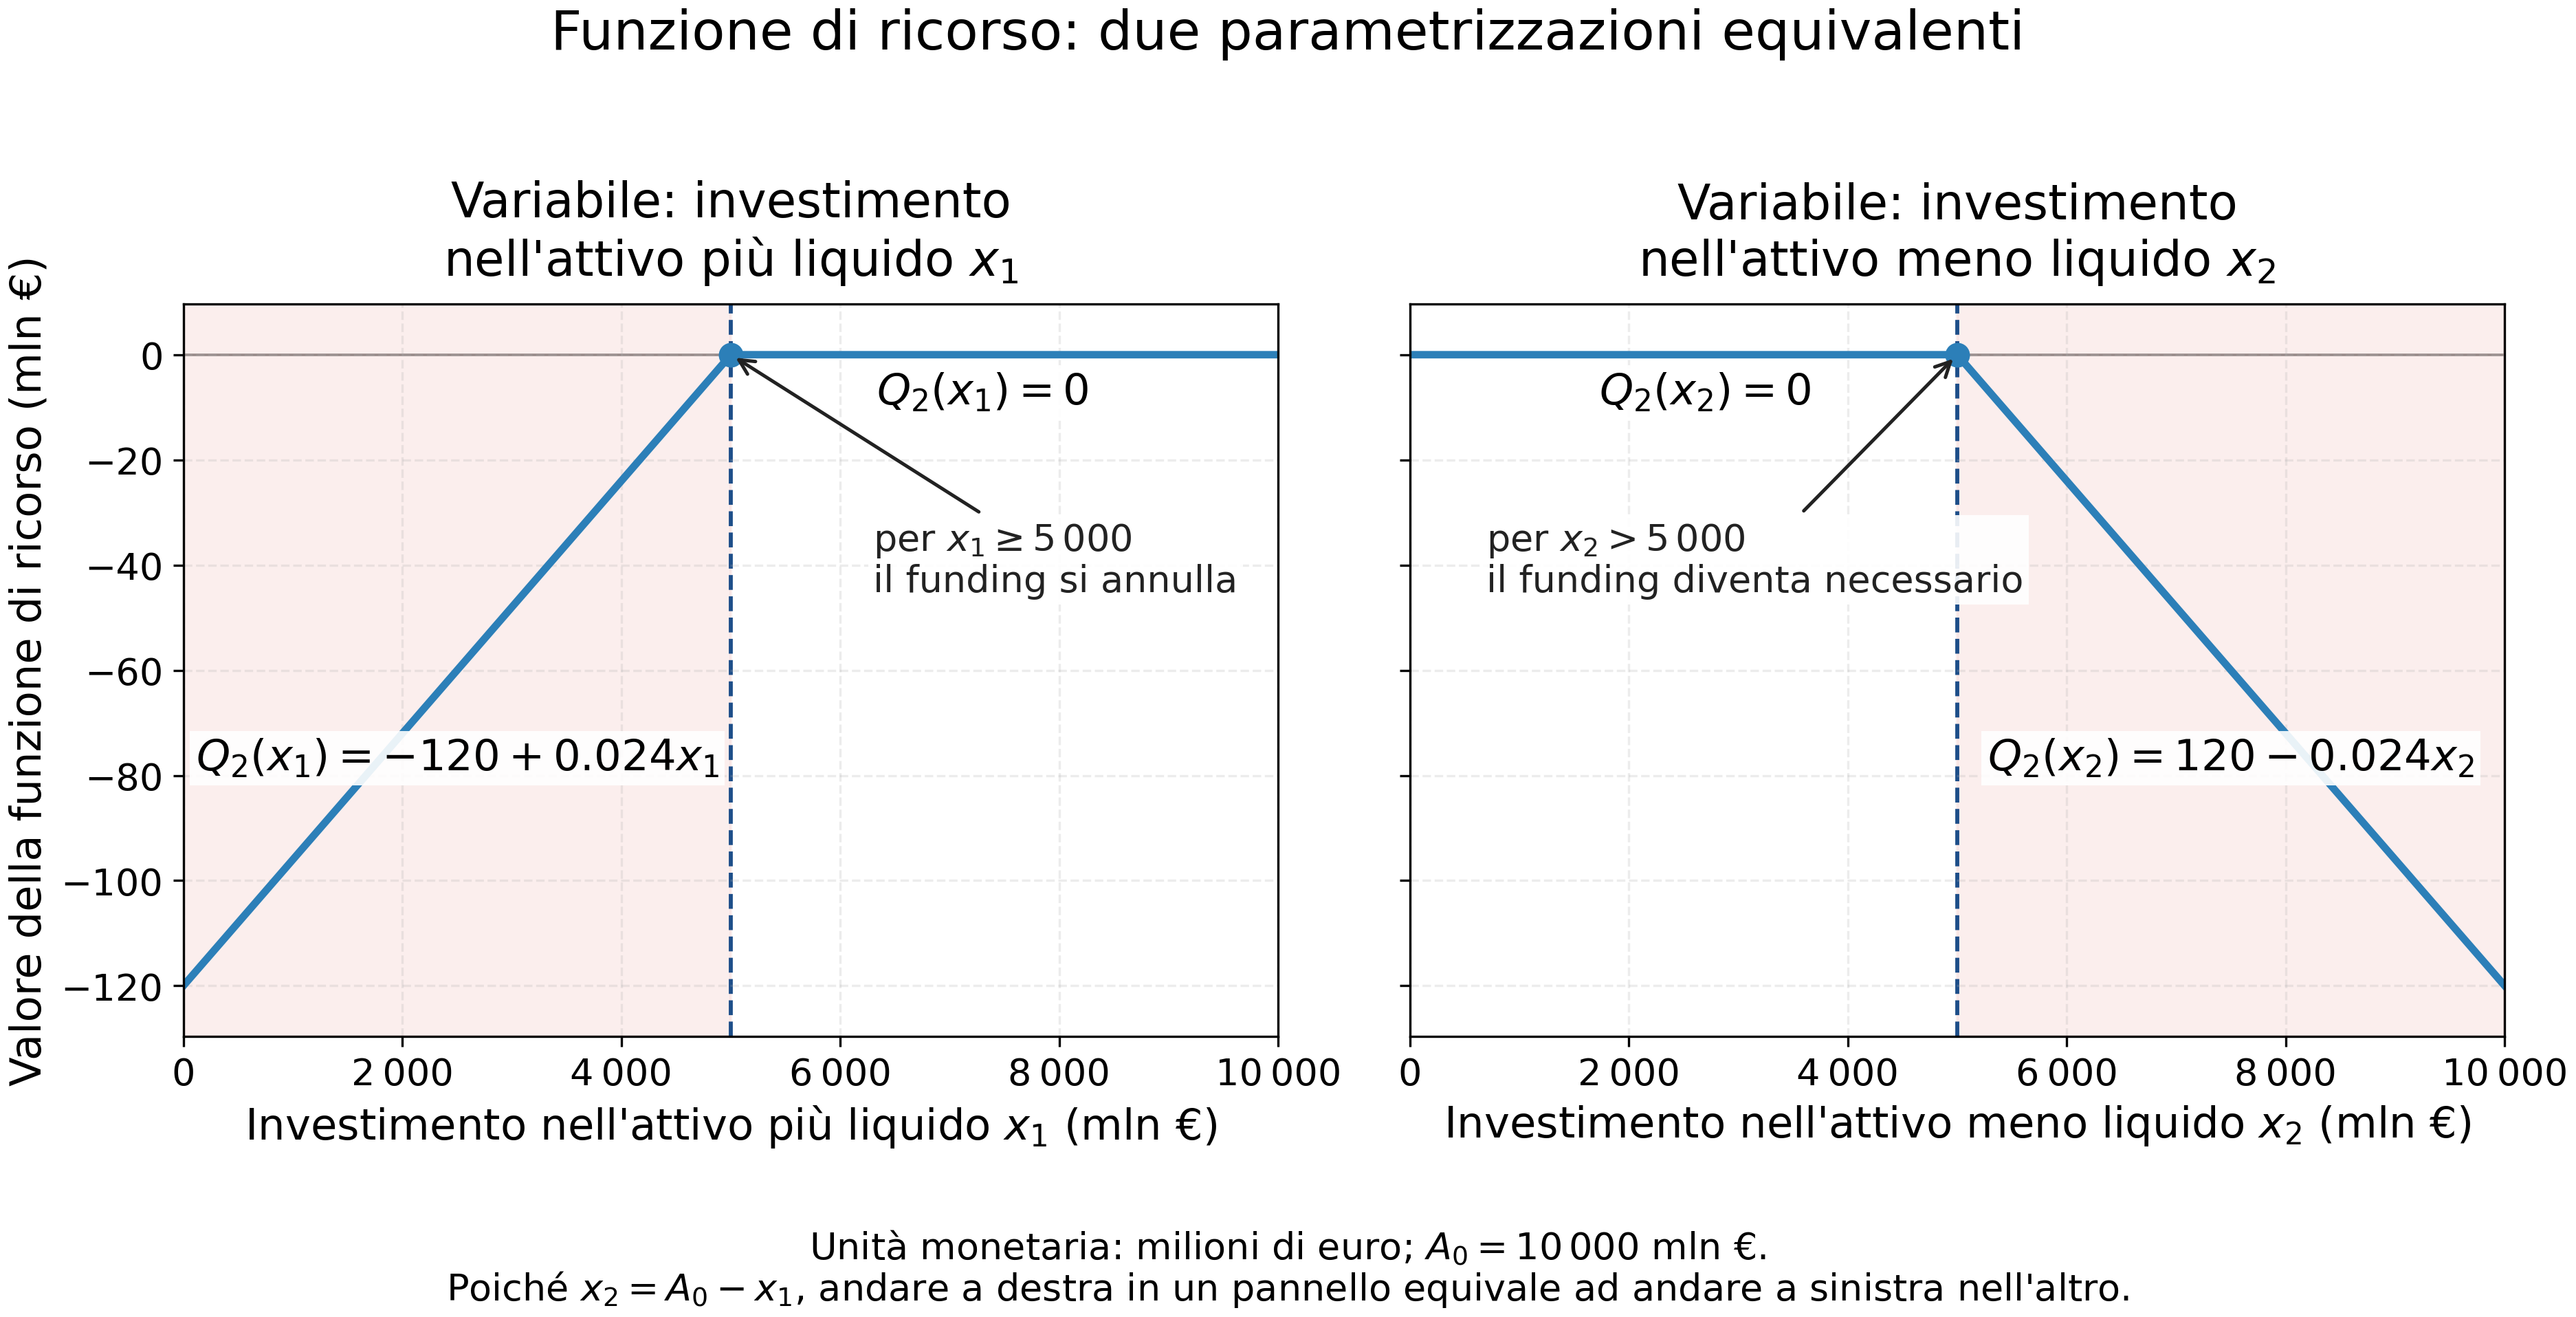
\includegraphics[width=0.80\textwidth]
{../graphics/Cap15_funzione_ricorso_piecewise.png}
\end{center}

\vspace{-3mm}

{\small
\begin{stepitemize}
\item A sinistra la variabile \`e $x_1$, a destra $x_2=10\,000-x_1$: stessi
portafogli. $Q_2$ cresce con l'attivo pi\`u liquido, decresce con l'altro.

\item Il punto angoloso ($x_1=x_2=5\,000$) segna il passaggio da funding
positivo a funding nullo.
\end{stepitemize}
}

%TCIMACRO{\TeXButton{Transition: Box Out}{\transboxout}}%
%BeginExpansion
\transboxout%
%EndExpansion
%TCIMACRO{\TeXButton{EndFrame}{\end{frame}}}%
%BeginExpansion
\end{frame}%
%EndExpansion

%****************************************

\section{Esercizio in aula: recourse con due scenari}

\subsection{La consegna}%

%TCIMACRO{\TeXButton{BeginFrame}{\begin{frame}}}%
%BeginExpansion
\begin{frame}%
%EndExpansion

\QTR{frametitle}{Esercizio: recourse con due scenari}

%TCIMACRO{\TeXButton{Transparency}{\setbeamercovered{transparent=20}}}%
%BeginExpansion
\setbeamercovered{transparent=20}%
%EndExpansion

{\footnotesize (Capitolo~14, Esercizio proposto~2)}

\medskip

Un intermediario assume al primo stadio $x=(5,\;5)'$. Il fabbisogno futuro
\`e $d=7$; due scenari con $p_1=0.7$ e $p_2=0.3$.

{\small
\[
a_1'=(1,\;0.9),
\qquad
a_2'=(1,\;0.3),
\qquad
a_s'x+u_s=d+g_s,
\qquad
g_s,u_s\geq0.
\]
}

Il costo unitario del funding \`e pari a $1$ nello scenario~1 e a $5$ nello
scenario~2.

\medskip

\begin{stepenumerate}
\item [1.] Scrivere $Q_1(x)$ e $Q_2(x)$.

\item [2.] Determinare $g_s^*$ e $u_s^*$ nei due scenari.

\item [3.] Calcolare $Q_1(x)$, $Q_2(x)$ e $\sum_{s\in\mathcal S}p_sQ_s(x)$.

\item [4.] Interpretare economicamente la differenza tra i valori delle due
funzioni di ricorso.
\end{stepenumerate}

%TCIMACRO{\TeXButton{Transition: Box Out}{\transboxout}}%
%BeginExpansion
\transboxout%
%EndExpansion
%TCIMACRO{\TeXButton{EndFrame}{\end{frame}}}%
%BeginExpansion
\end{frame}%
%EndExpansion

%****************************************

\subsection{La soluzione}%

%TCIMACRO{\TeXButton{BeginFrame}{\begin{frame}}}%
%BeginExpansion
\begin{frame}%
%EndExpansion

\QTR{frametitle}{Soluzione: stessa decisione, ricorsi diversi}

%TCIMACRO{\TeXButton{Transparency}{\setbeamercovered{transparent=20}}}%
%BeginExpansion
\setbeamercovered{transparent=20}%
%EndExpansion

\begin{stepenumerate}
\item [1.] {\small $Q_1(x)=\max\{-u_1:\;x_1+0.9x_2+u_1=7+g_1,\ g_1,u_1\geq0\}$,
\newline
$Q_2(x)=\max\{-5u_2:\;x_1+0.3x_2+u_2=7+g_2,\ g_2,u_2\geq0\}$.}

\item [2.] Scenario~1: liquidit\`a $5+4.5=9.5>7$, quindi $g_1^*=2.5$ e
$u_1^*=0$. Scenario~2: liquidit\`a $5+1.5=6.5<7$, quindi $g_2^*=0$ e
$u_2^*=0.5$.

\item [3.] $Q_1(x)=0$, $\;Q_2(x)=-5\cdot0.5=-2.5$,
\[
\sum_{s\in\mathcal S}p_sQ_s(x)=0.7\cdot0+0.3\cdot(-2.5)=-0.75.
\]

\item [4.] La stessa $x$ lascia un'eccedenza nello scenario~1 e un deficit
nello scenario~2, dove il funding \`e anche pi\`u costoso.
\end{stepenumerate}

\medskip

\begin{center}
{\small Il valore di una decisione iniziale dipende da come si comporta in
\textbf{tutti} gli scenari.}
\end{center}

%TCIMACRO{\TeXButton{Transition: Box Out}{\transboxout}}%
%BeginExpansion
\transboxout%
%EndExpansion
%TCIMACRO{\TeXButton{EndFrame}{\end{frame}}}%
%BeginExpansion
\end{frame}%
%EndExpansion

%****************************************

\section{Esercizio in aula: scelta ottima e scenario avverso}

\subsection{La consegna}%

%TCIMACRO{\TeXButton{BeginFrame}{\begin{frame}}}%
%BeginExpansion
\begin{frame}%
%EndExpansion

\QTR{frametitle}{Esercizio: scelta ottima e probabilit\`a dello scenario avverso}

%TCIMACRO{\TeXButton{Transparency}{\setbeamercovered{transparent=20}}}%
%BeginExpansion
\setbeamercovered{transparent=20}%
%EndExpansion

{\footnotesize (Capitolo~14, Esercizio proposto~3)}

\medskip

{\small Risorse iniziali $A_0=10$, con $x_1+x_2=10$ e $x_1,x_2\geq0$; contributo
economico di primo stadio $c'x=x_1+2x_2$. Il primo attivo produce sempre una
unit\`a di liquidit\`a per unit\`a investita; il secondo produce $0.8$ nel primo
scenario e $0.2$ nel secondo. Fabbisogno $d=6$; costo unitario del funding $1$
nel primo scenario e $6$ nel secondo; $p$ \`e la probabilit\`a dello scenario
avverso.}

\medskip

\begin{stepenumerate}
\item [1.] Determinare le funzioni di ricorso dei due scenari come funzioni di
$x_2$.

\item [2.] Scrivere la funzione obiettivo complessiva come funzione di $x_2$ e
di $p$.

\item [3.] Determinare per quali valori di $p$ l'allocazione $x_2=10$ \`e
preferibile all'allocazione $x_2=5$.

\item [4.] Interpretare il risultato in termini di compromesso tra maggiore
redditivit\`a iniziale e costo atteso del ricorso.
\end{stepenumerate}

%TCIMACRO{\TeXButton{Transition: Box Out}{\transboxout}}%
%BeginExpansion
\transboxout%
%EndExpansion
%TCIMACRO{\TeXButton{EndFrame}{\end{frame}}}%
%BeginExpansion
\end{frame}%
%EndExpansion

%****************************************

\subsection{La soluzione: ricorso e obiettivo}%

%TCIMACRO{\TeXButton{BeginFrame}{\begin{frame}}}%
%BeginExpansion
\begin{frame}%
%EndExpansion

\QTR{frametitle}{Soluzione: ricorso e obiettivo in funzione di $x_2$}

%TCIMACRO{\TeXButton{Transparency}{\setbeamercovered{transparent=20}}}%
%BeginExpansion
\setbeamercovered{transparent=20}%
%EndExpansion

Con $x_1=10-x_2$:

\begin{stepenumerate}
\item [1.] Scenario~1: liquidit\`a $10-0.2x_2\geq8>6$, quindi non serve
funding e $Q_1(x_2)=0$.

Scenario~2: liquidit\`a $10-0.8x_2$; il deficit \`e $0.8x_2-4$ quando
positivo:
\[
Q_2(x_2)=-6\max\{0,\;0.8x_2-4\}.
\]

\item [2.] Con $c'x=x_1+2x_2=10+x_2$:
\[
V(x_2;p)=10+x_2-6p\max\{0,\;0.8x_2-4\}.
\]
\end{stepenumerate}

\medskip

{\small $Q_2$ \`e concava e lineare a tratti, con punto angoloso in $x_2=5$:
\`e la propriet\`a della funzione di ricorso vista poco fa.}

%TCIMACRO{\TeXButton{Transition: Box Out}{\transboxout}}%
%BeginExpansion
\transboxout%
%EndExpansion
%TCIMACRO{\TeXButton{EndFrame}{\end{frame}}}%
%BeginExpansion
\end{frame}%
%EndExpansion

%****************************************

\subsection{La soluzione: il confronto}%

%TCIMACRO{\TeXButton{BeginFrame}{\begin{frame}}}%
%BeginExpansion
\begin{frame}%
%EndExpansion

\QTR{frametitle}{Soluzione: dove si rompe il compromesso}

%TCIMACRO{\TeXButton{Transparency}{\setbeamercovered{transparent=20}}}%
%BeginExpansion
\setbeamercovered{transparent=20}%
%EndExpansion

\begin{stepenumerate}
\item [3.] Per le due allocazioni richieste
\[
V(10;p)=20-24p,
\qquad
V(5;p)=15,
\]
quindi
\[
x_2=10\ \text{\`e preferibile a}\ x_2=5
\iff
p<\frac{5}{24}\approx0.2083.
\]
Per $p=5/24$ le due allocazioni sono equivalenti.

\item [4.] Passare da $x_2=5$ a $x_2=10$ aumenta il contributo iniziale di $5$,
ma nello scenario avverso richiede $4$ unit\`a di funding al costo unitario
$6$: un costo atteso pari a $24p$.
\end{stepenumerate}

\medskip

\begin{center}
{\small Il portafoglio pi\`u redditizio conviene solo se lo scenario avverso
\`e abbastanza improbabile.}

\medskip

{\small \textbf{Domanda per la pausa}: che cosa accadrebbe scegliendo $x$ con
il solo scenario medio?}
\end{center}

%TCIMACRO{\TeXButton{Transition: Box Out}{\transboxout}}%
%BeginExpansion
\transboxout%
%EndExpansion
%TCIMACRO{\TeXButton{EndFrame}{\end{frame}}}%
%BeginExpansion
\end{frame}%
%EndExpansion

%****************************************

\section{Tre modi di scegliere la decisione iniziale}

\subsection{Tre benchmark}%

%TCIMACRO{\TeXButton{BeginFrame}{\begin{frame}}}%
%BeginExpansion
\begin{frame}%
%EndExpansion

\QTR{frametitle}{Tre benchmark, tre ipotesi informative}

%TCIMACRO{\TeXButton{Transparency}{\setbeamercovered{transparent=20}}}%
%BeginExpansion
\setbeamercovered{transparent=20}%
%EndExpansion

Per interpretare la programmazione stocastica si confrontano tre valori di
riferimento:
\[
z^{SP},
\qquad
z^{WS},
\qquad
z^{EV}.
\]

{\small
\begin{center}
\begin{tabular}{l|p{3.3cm}|p{4.6cm}}
\hline
& \textbf{Quando si sceglie $x$} & \textbf{Con quale informazione}\\
\hline
SP & prima dello scenario & la distribuzione degli scenari\\
WS & dopo lo scenario & lo scenario, noto in anticipo\\
EV & prima dello scenario & i soli valori medi dei dati\\
\hline
\end{tabular}
\end{center}
}

\medskip

\begin{stepitemize}
\item I tre valori separano due vantaggi economici: la \textbf{conoscenza
anticipata} del futuro e l'\textbf{uso della distribuzione} degli scenari nella
scelta iniziale.

\item Risposta alla domanda della pausa: \`e il benchmark EV.
\end{stepitemize}

%TCIMACRO{\TeXButton{Transition: Box Out}{\transboxout}}%
%BeginExpansion
\transboxout%
%EndExpansion
%TCIMACRO{\TeXButton{EndFrame}{\end{frame}}}%
%BeginExpansion
\end{frame}%
%EndExpansion

%****************************************

\subsection{SP e WS}%

%TCIMACRO{\TeXButton{BeginFrame}{\begin{frame}}}%
%BeginExpansion
\begin{frame}%
%EndExpansion

\QTR{frametitle}{Massimo del valore atteso o valore atteso dei massimi}

%TCIMACRO{\TeXButton{Transparency}{\setbeamercovered{transparent=20}}}%
%BeginExpansion
\setbeamercovered{transparent=20}%
%EndExpansion

\textbf{Soluzione stocastica (SP)}: un unico $x$, comune a tutti gli scenari,
{\small
\[
z^{SP}
=
\max_{x\in\mathcal X_0}
\Big\{
c'x+\sum_{s\in\mathcal S}p_sQ_s(x)
\Big\}.
\]
}

\textbf{Soluzione wait-and-see (WS)}: lo scenario \`e noto prima di scegliere
anche $x$, quindi un $x_s$ per scenario,
{\small
\[
z^{WS}
=
\sum_{s\in\mathcal S}p_s
\max_{x_s\in\mathcal X_0}
\big\{
c'x_s+Q_s(x_s)
\big\}.
\]
}

\begin{stepitemize}
\item In SP si massimizza un valore atteso; in WS si calcola il valore atteso
dei massimi.

\item Nel modello a due stadi la differenza riguarda soltanto la decisione
iniziale: in entrambi il ricorso conosce lo scenario completo.
\end{stepitemize}

%TCIMACRO{\TeXButton{Transition: Box Out}{\transboxout}}%
%BeginExpansion
\transboxout%
%EndExpansion
%TCIMACRO{\TeXButton{EndFrame}{\end{frame}}}%
%BeginExpansion
\end{frame}%
%EndExpansion

%****************************************

\subsection{Il problema medio}%

%TCIMACRO{\TeXButton{BeginFrame}{\begin{frame}}}%
%BeginExpansion
\begin{frame}%
%EndExpansion

\QTR{frametitle}{Il problema medio e la decisione $x^{EV}$}

%TCIMACRO{\TeXButton{Transparency}{\setbeamercovered{transparent=20}}}%
%BeginExpansion
\setbeamercovered{transparent=20}%
%EndExpansion

I coefficienti incerti vengono sostituiti dai rispettivi valori attesi:
{\small
\[
\bar q=\sum_sp_sq_s,
\qquad
\bar T=\sum_sp_sT_s,
\qquad
\bar W=\sum_sp_sW_s,
\qquad
\bar h=\sum_sp_sh_s.
\]
\[
\bar Q(x)
=
\max_{\bar y\in\bar{\mathcal Y}}
\left\{
\bar q'\bar y:\;
\bar Tx+\bar W\bar y=\bar h
\right\},
\qquad
\boxed{
x^{EV}\in\arg\max_{x\in\mathcal X_0}
\left\{
c'x+\bar Q(x)
\right\}.}
\]
}

\begin{stepitemize}
\item $x^{EV}$ \textbf{non} si ottiene mediando le decisioni ottime dei singoli
scenari: \`e la soluzione di un nuovo programma lineare, costruito con i dati
medi.

\item Nel caso SVB-ALM: $\bar a_{tj}=\sum_sp_sa_{tj}^s$ e
$\bar d_t=\sum_sp_sd_t^s$; lo stesso criterio vale per gli altri coefficienti
incerti e per i limiti di funding.
\end{stepitemize}

%TCIMACRO{\TeXButton{Transition: Box Out}{\transboxout}}%
%BeginExpansion
\transboxout%
%EndExpansion
%TCIMACRO{\TeXButton{EndFrame}{\end{frame}}}%
%BeginExpansion
\end{frame}%
%EndExpansion

%****************************************

\subsection{La valutazione della decisione EV}%

%TCIMACRO{\TeXButton{BeginFrame}{\begin{frame}}}%
%BeginExpansion
\begin{frame}%
%EndExpansion

\QTR{frametitle}{Valutare $x^{EV}$ negli scenari originari}

%TCIMACRO{\TeXButton{Transparency}{\setbeamercovered{transparent=20}}}%
%BeginExpansion
\setbeamercovered{transparent=20}%
%EndExpansion

\textbf{Prima operazione.} Con $x=x^{EV}$ fissato, si risolve il problema di
ricorso in ciascuno scenario, con i suoi coefficienti:
{\small
\[
Q_s(x^{EV})
=
\max_{y_s\in\mathcal X_s}
\left\{
q_s'y_s:\;
T_sx^{EV}+W_sy_s=h_s
\right\}.
\]
}

\textbf{Seconda operazione.} Si aggregano i valori con le probabilit\`a degli
scenari:
{\small
\[
\boxed{
z^{EV}
=
c'x^{EV}
+
\sum_{s\in\mathcal S}p_sQ_s(x^{EV}).}
\]
}

\begin{stepitemize}
\item Non si utilizzano le decisioni di ricorso del problema medio.

\item \textbf{$z^{EV}$ non coincide, in generale, con il valore ottimo del
problema medio}: \`e l'errore pi\`u frequente.
\end{stepitemize}

%TCIMACRO{\TeXButton{Transition: Box Out}{\transboxout}}%
%BeginExpansion
\transboxout%
%EndExpansion
%TCIMACRO{\TeXButton{EndFrame}{\end{frame}}}%
%BeginExpansion
\end{frame}%
%EndExpansion

%****************************************

\subsection{EVPI e VSS}%

%TCIMACRO{\TeXButton{BeginFrame}{\begin{frame}}}%
%BeginExpansion
\begin{frame}%
%EndExpansion

\QTR{frametitle}{Ordinamento, EVPI e VSS}

%TCIMACRO{\TeXButton{Transparency}{\setbeamercovered{transparent=20}}}%
%BeginExpansion
\setbeamercovered{transparent=20}%
%EndExpansion

Per problemi di massimizzazione, con benchmark ben definiti e $x^{EV}$ che
ammette ricorso:
{\small
\[
z^{WS}\geq z^{SP}\geq z^{EV},
\qquad
\EVPI=z^{WS}-z^{SP}\geq0,
\qquad
\VSS=z^{SP}-z^{EV}\geq0.
\]
}

\vspace{-2mm}

\begin{center}
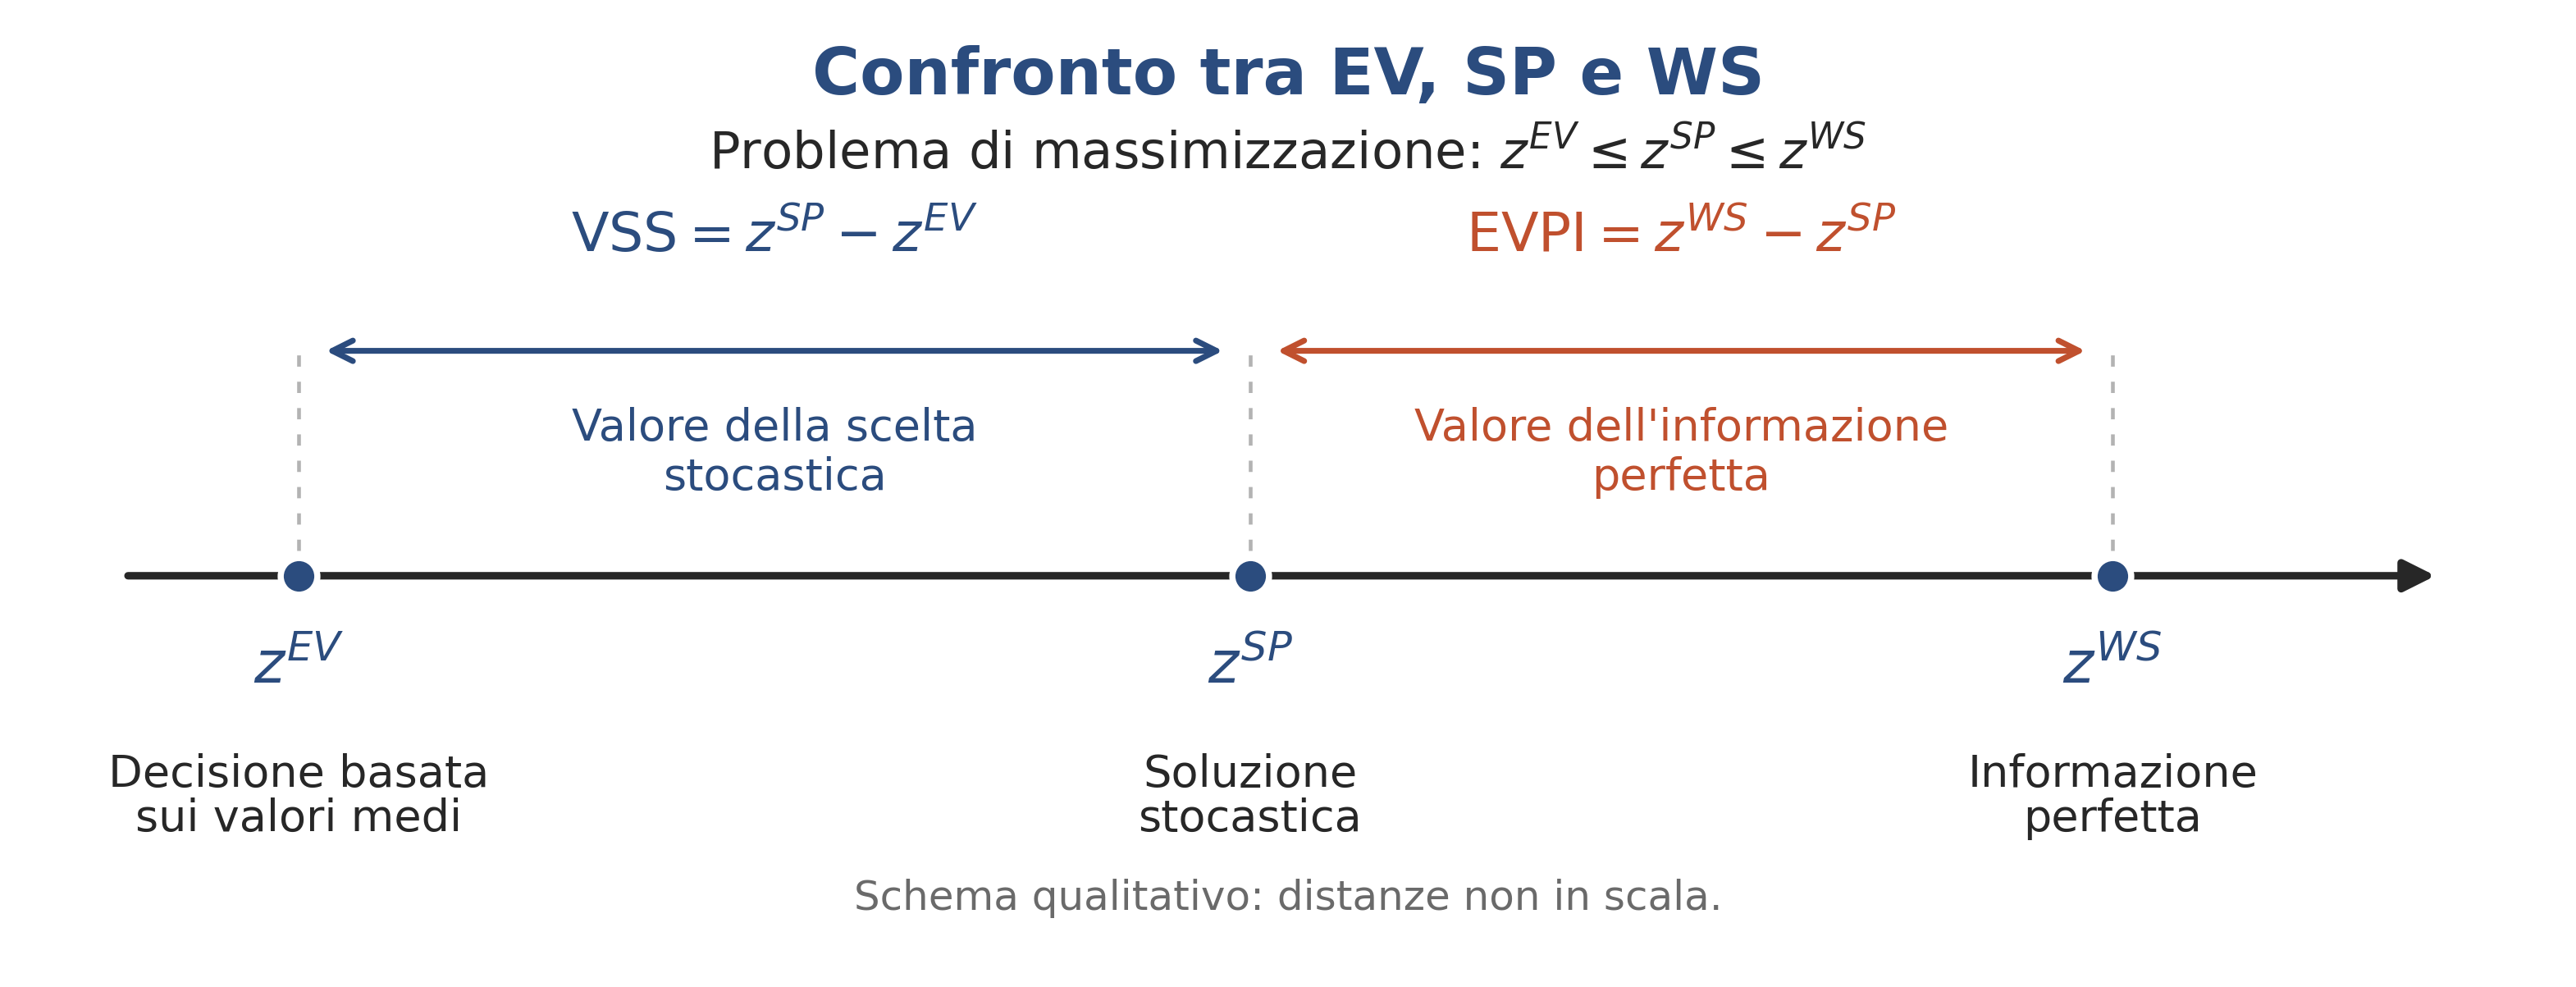
\includegraphics[width=0.55\textwidth]
{../graphics/Cap15_confronto_SP_EV_WS.png}
\end{center}

\vspace{-2mm}

{\small
\begin{center}
\begin{tabular}{l|l}
\hline
$\EVPI$ & quanto vale conoscere perfettamente il futuro?\\
$\VSS$ & quanto vale utilizzare il modello stocastico?\\
\hline
\end{tabular}
\end{center}
}

{\footnotesize Lo schema \`e qualitativo. Non esiste un ordine generale fra
$\EVPI$ e $\VSS$: uno dei due pu\`o essere nullo anche quando l'altro \`e
positivo.}

%TCIMACRO{\TeXButton{Transition: Box Out}{\transboxout}}%
%BeginExpansion
\transboxout%
%EndExpansion
%TCIMACRO{\TeXButton{EndFrame}{\end{frame}}}%
%BeginExpansion
\end{frame}%
%EndExpansion

%****************************************

\section{Esercizio in aula: valore dell'informazione e della soluzione stocastica}

\subsection{La consegna}%

%TCIMACRO{\TeXButton{BeginFrame}{\begin{frame}}}%
%BeginExpansion
\begin{frame}%
%EndExpansion

\QTR{frametitle}{Esercizio: valore dell'informazione e della soluzione stocastica}

%TCIMACRO{\TeXButton{Transparency}{\setbeamercovered{transparent=20}}}%
%BeginExpansion
\setbeamercovered{transparent=20}%
%EndExpansion

{\footnotesize (Capitolo~15, Esercizio svolto~3)}

\smallskip

{\footnotesize Una banca dispone di $10$ milioni di euro da allocare fra cassa e
riserve ($x_1$, rendimento unitario $0.01$) e titoli meno liquidi ($x_2$,
rendimento unitario $0.05$): $x_1+x_2=10$, $x_1,x_2\geq0$. Alla data futura deve
soddisfare un fabbisogno di liquidit\`a pari a $8$ milioni; dopo lo scenario
pu\`o raccogliere funding $u_s$, con $0\leq u_s\leq3$, o mantenere una giacenza
$g_s\geq0$. Due scenari equiprobabili, $p_1=p_2=0.5$, con coefficienti di
liquidit\`a $a_1'=(1,\;0.9)$ e $a_2'=(1,\;0.5)$; costo unitario del funding
$\gamma_1=0.02$ e $\gamma_2=0.20$.}

\smallskip

{\footnotesize
\begin{stepenumerate}
\item [1.] Formulare i problemi di ricorso $Q_s(x)$ e identificare $T_s$,
$W_s$, $h_s$ e $q_s$.

\item [2.] Determinare le funzioni di ricorso e risolvere il problema
stocastico, calcolando $x^{SP}$ e $z^{SP}$.

\item [3.] Risolvere i problemi wait-and-see nei due scenari e calcolare
$z^{WS}$.

\item [4.] Costruire il problema deterministico medio, determinare $x^{EV}$ e
calcolare $z^{EV}$ valutando $x^{EV}$ negli scenari originari.

\item [5.] Calcolare EVPI e VSS, verificare l'ordinamento dei tre valori e
interpretare economicamente i risultati.
\end{stepenumerate}
}

%TCIMACRO{\TeXButton{Transition: Box Out}{\transboxout}}%
%BeginExpansion
\transboxout%
%EndExpansion
%TCIMACRO{\TeXButton{EndFrame}{\end{frame}}}%
%BeginExpansion
\end{frame}%
%EndExpansion

%****************************************

\subsection{La soluzione stocastica}%

%TCIMACRO{\TeXButton{BeginFrame}{\begin{frame}}}%
%BeginExpansion
\begin{frame}%
%EndExpansion

\QTR{frametitle}{Soluzione: il programma stocastico}

%TCIMACRO{\TeXButton{Transparency}{\setbeamercovered{transparent=20}}}%
%BeginExpansion
\setbeamercovered{transparent=20}%
%EndExpansion

{\small
\[
Q_s(x)=\max_{\substack{g_s\geq0\\0\leq u_s\leq3}}
\left\{-\gamma_su_s:\;a_s'x+u_s-g_s=8\right\}
\]
}

\vspace{-2mm}

{\footnotesize Nella forma $T_sx+W_sy_s=h_s$: $T_s=(1\;\;a_{s2})$,
$W_s=(-1\;\;1)$, $h_s=8$, $q_s=(0,\;-\gamma_s)'$.}

{\footnotesize
\begin{stepitemize}
\item Scenario~1: $a_1'x=10-0.1x_2\geq9>8$, il funding non \`e mai necessario,
$Q_1=0$. Scenario~2: $a_2'x=10-0.5x_2$, quindi $u_2^*=\max\{0,\;0.5x_2-2\}$ e
$Q_2=-0.20\,u_2^*$.

\item Funzione obiettivo ridotta: $\Pi^{SP}(x_2)=0.10+0.04x_2$ fino a $x_2=4$,
poi $0.30-0.01x_2$.
\end{stepitemize}
}

\vspace{-2mm}

\begin{center}
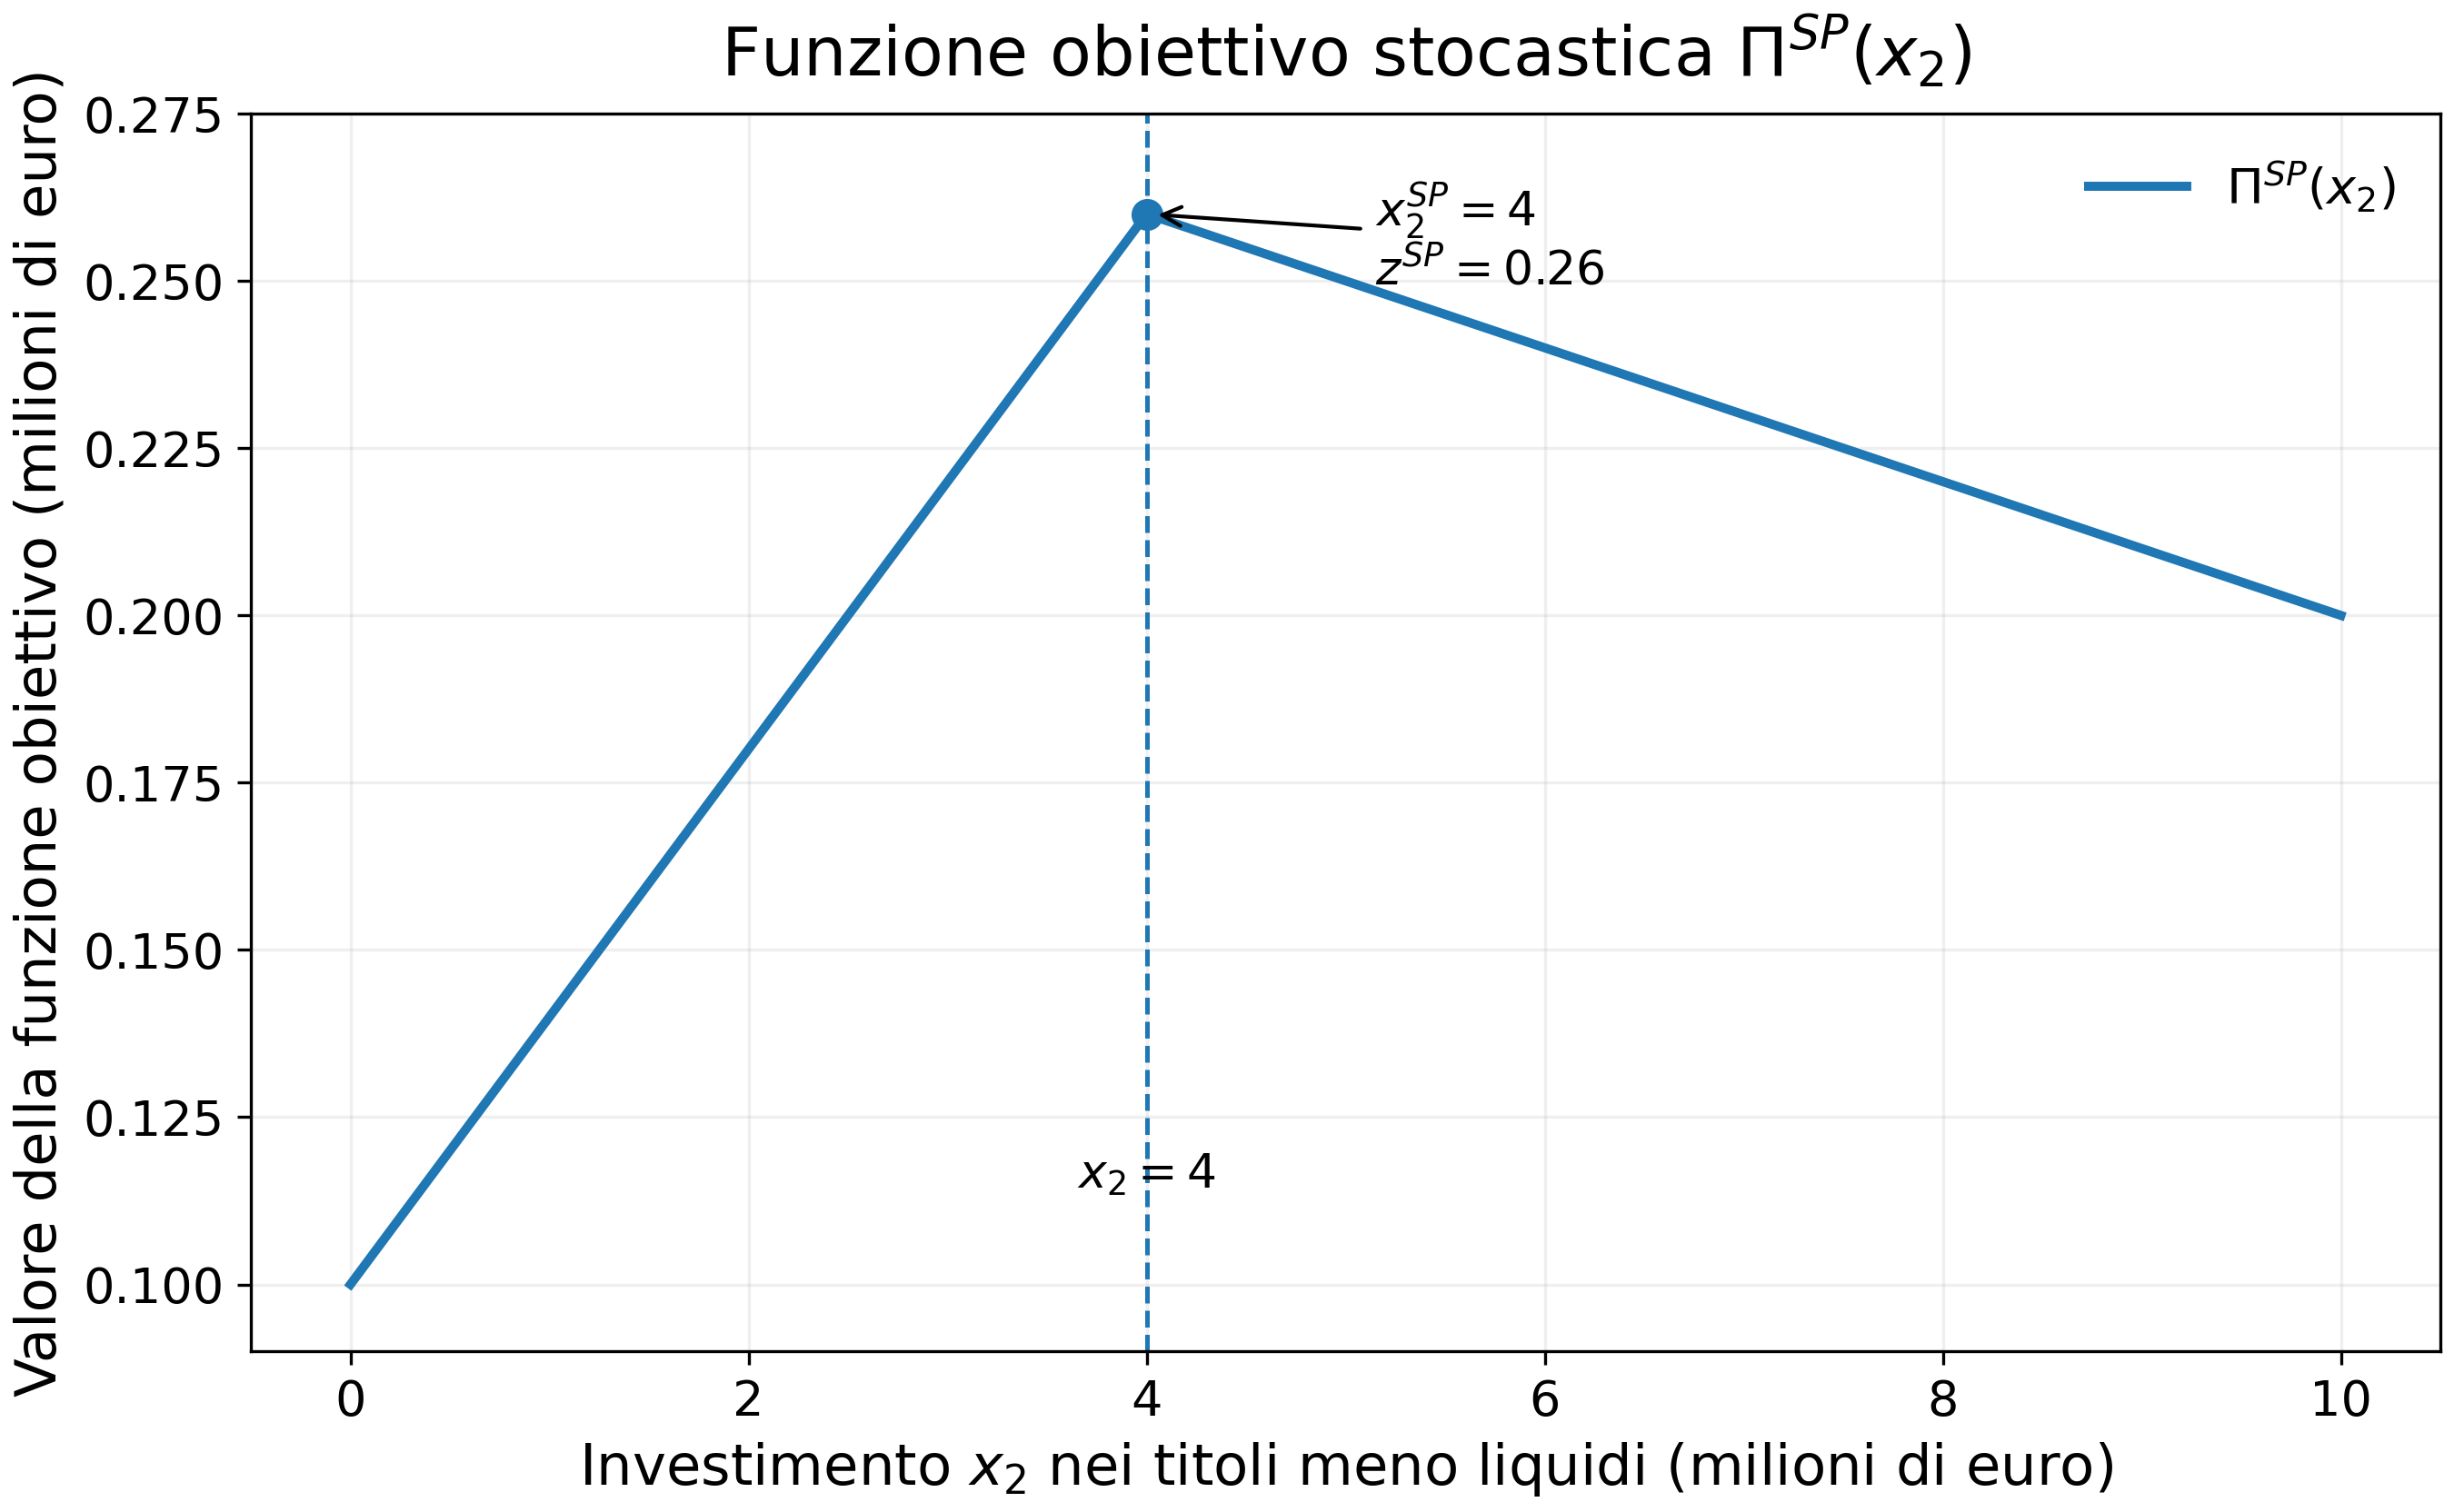
\includegraphics[width=0.44\textwidth]
{../graphics/Cap15_funzione_obiettivo_SP.png}
\end{center}

\vspace{-4mm}

\begin{center}
{\small $x^{SP}=(6,\;4)'$, $\qquad z^{SP}=0.26$}
\end{center}

%TCIMACRO{\TeXButton{Transition: Box Out}{\transboxout}}%
%BeginExpansion
\transboxout%
%EndExpansion
%TCIMACRO{\TeXButton{EndFrame}{\end{frame}}}%
%BeginExpansion
\end{frame}%
%EndExpansion

%****************************************

\subsection{WS ed EV}%

%TCIMACRO{\TeXButton{BeginFrame}{\begin{frame}}}%
%BeginExpansion
\begin{frame}%
%EndExpansion

\QTR{frametitle}{Soluzione: wait-and-see e valori medi}

%TCIMACRO{\TeXButton{Transparency}{\setbeamercovered{transparent=20}}}%
%BeginExpansion
\setbeamercovered{transparent=20}%
%EndExpansion

{\footnotesize
\textbf{WS}: scenario~1, ottimo $0.50$ con $x_2=10$; scenario~2, ottimo $0.26$
con $x_2=4$; quindi $z^{WS}=0.5(0.50)+0.5(0.26)=0.38$.

\smallskip

\textbf{EV}: $\bar a_2=0.7$ e $\bar\gamma=0.11$; il funding parte da
$x_2=20/3$ e $\Pi^{EV}(x_2)$ resta crescente.}

\vspace{-2mm}

\begin{center}
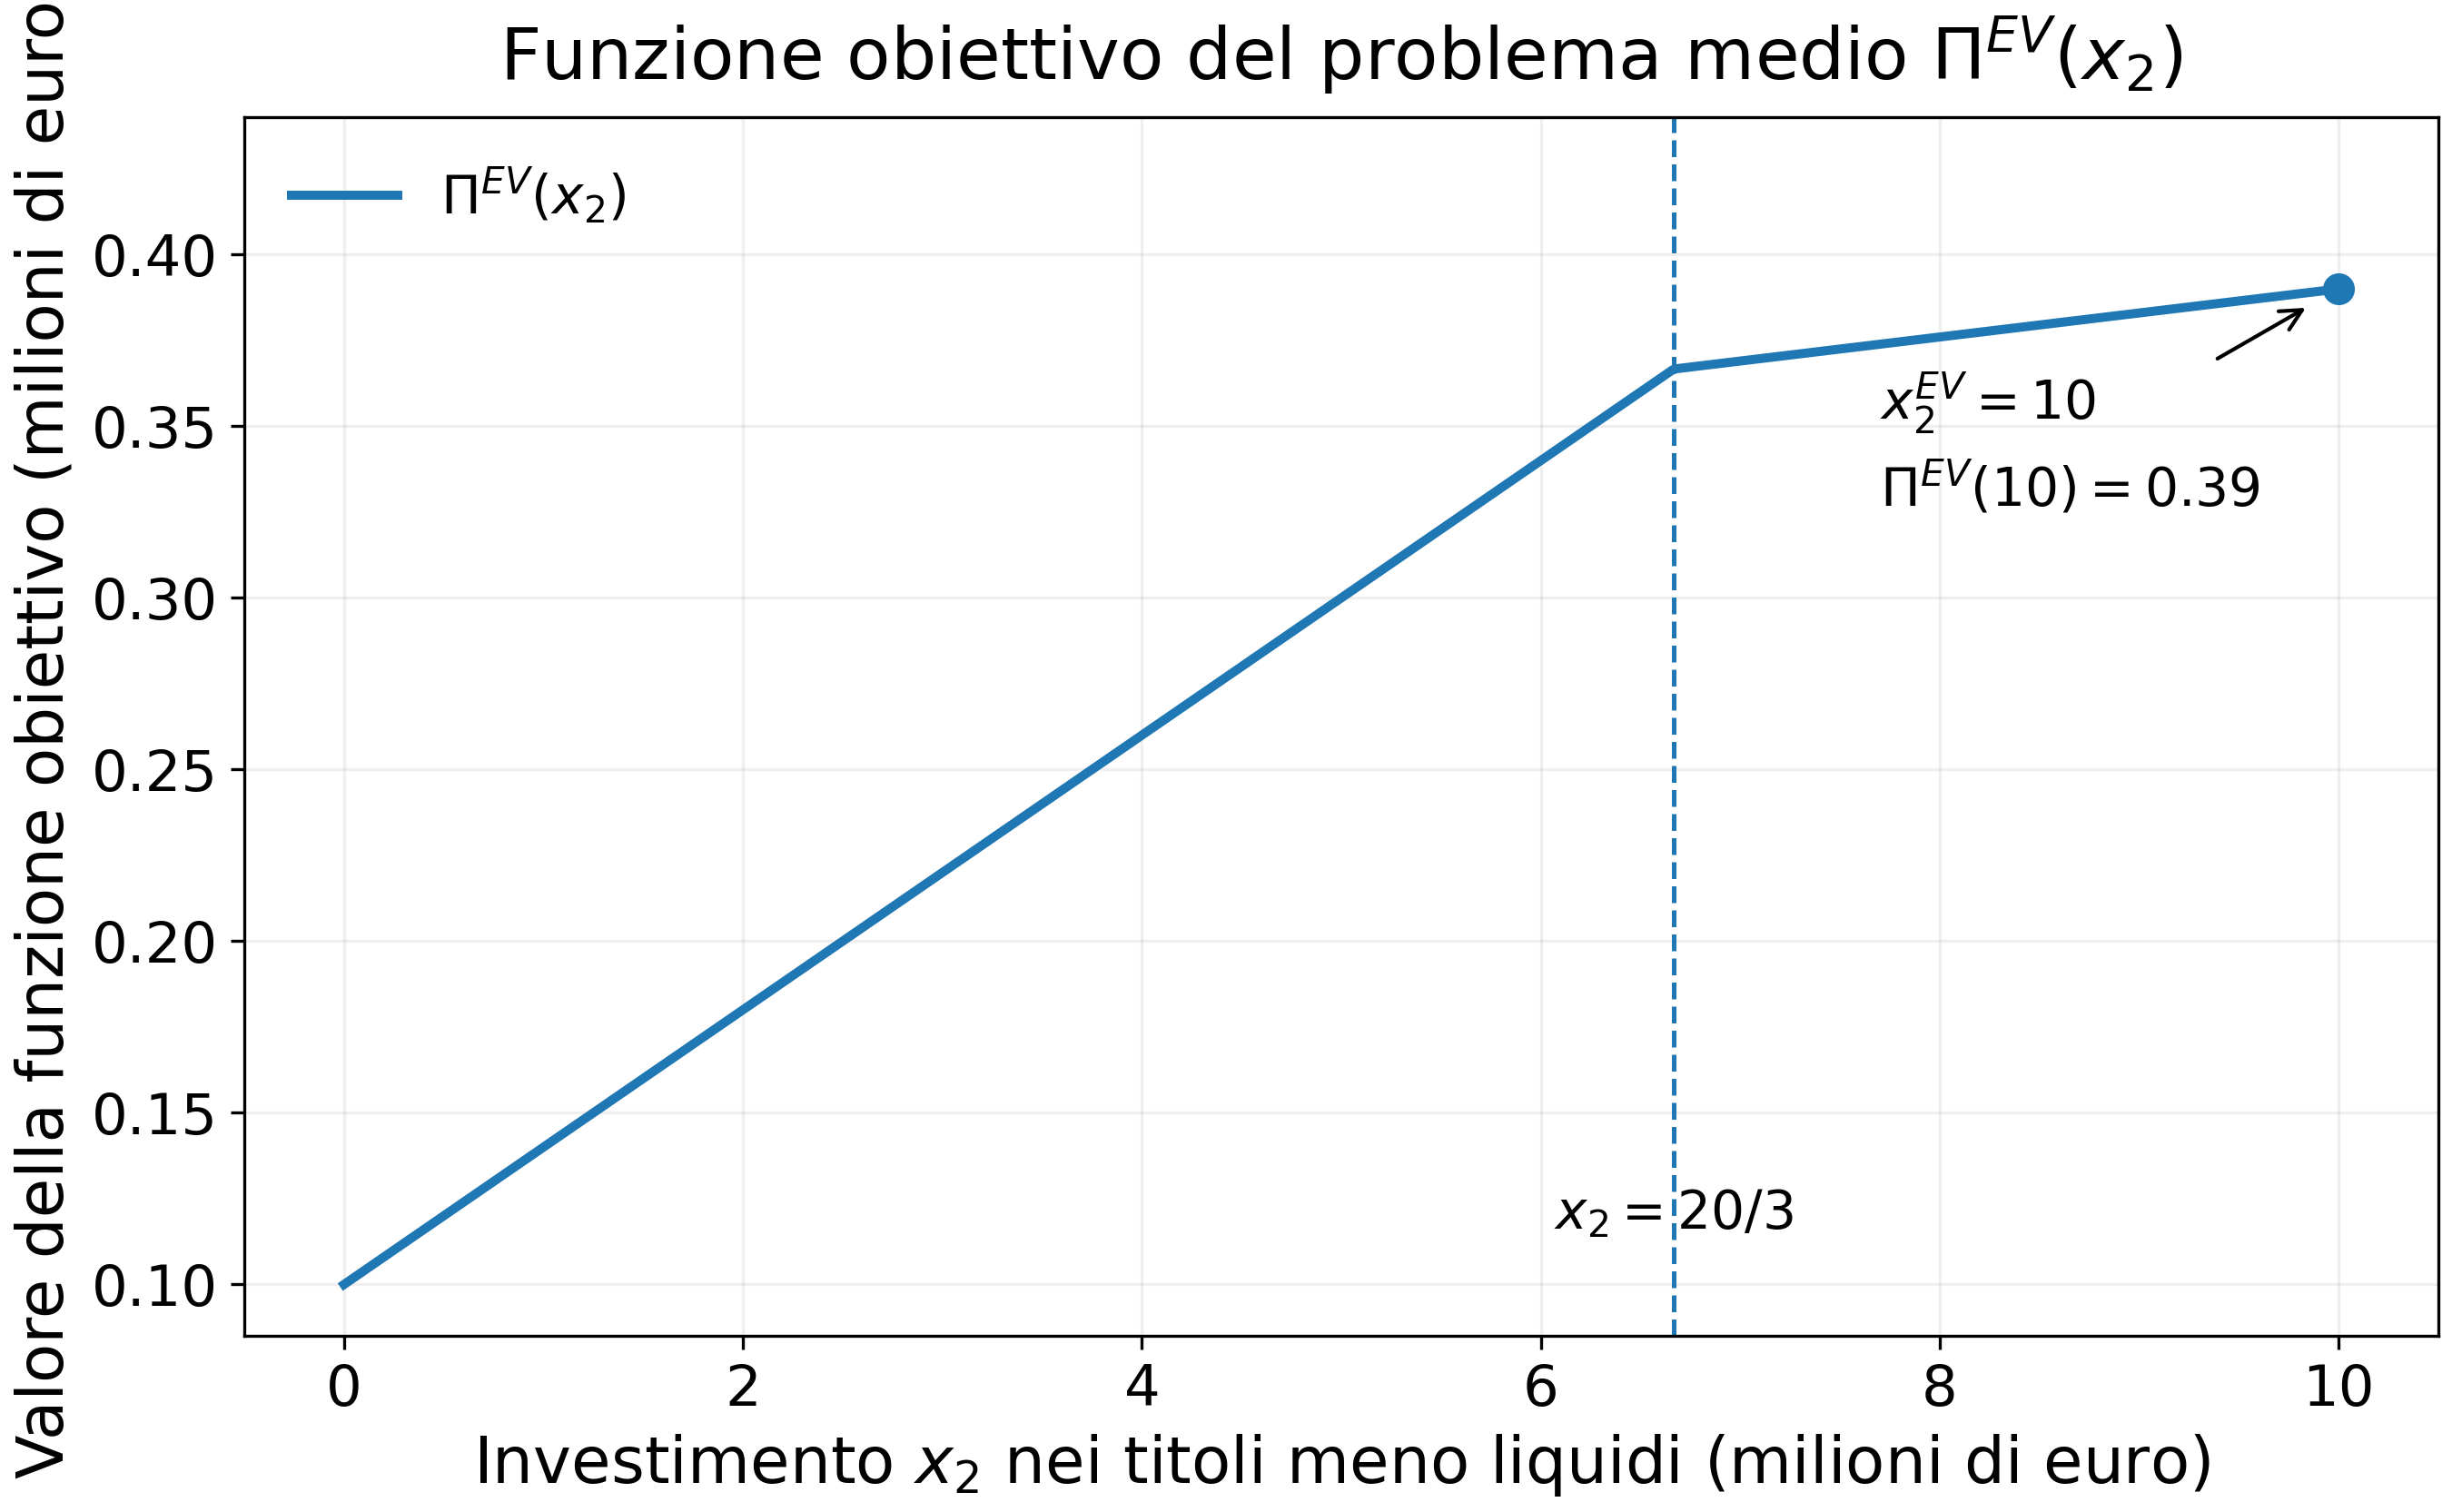
\includegraphics[width=0.44\textwidth]
{../graphics/Cap15_funzione_obiettivo_EV.png}
\end{center}

\vspace{-4mm}

{\footnotesize
\[
x^{EV}=(0,\;10)',
\qquad
\Pi^{EV}(10)=0.39\ \text{(ottimo del problema medio)}.
\]

\vspace{-1mm}

Valutando $x^{EV}$ negli scenari originari: $Q_1=0$; nello scenario~2 il
deficit \`e $3$ e satura il funding, $Q_2=-0.60$. Quindi
$z^{EV}=0.50+\tfrac12(0)+\tfrac12(-0.60)=\mathbf{0.20}$.}

%TCIMACRO{\TeXButton{Transition: Box Out}{\transboxout}}%
%BeginExpansion
\transboxout%
%EndExpansion
%TCIMACRO{\TeXButton{EndFrame}{\end{frame}}}%
%BeginExpansion
\end{frame}%
%EndExpansion

%****************************************

\subsection{Interpretazione}%

%TCIMACRO{\TeXButton{BeginFrame}{\begin{frame}}}%
%BeginExpansion
\begin{frame}%
%EndExpansion

\QTR{frametitle}{Che cosa misurano i numeri}

%TCIMACRO{\TeXButton{Transparency}{\setbeamercovered{transparent=20}}}%
%BeginExpansion
\setbeamercovered{transparent=20}%
%EndExpansion

{\small
\renewcommand{\arraystretch}{1.25}
\begin{center}
\begin{tabular}{lcc}
\hline
& \textbf{valore} & \textbf{decisione iniziale}\\
\hline
$z^{WS}$ & $0.38$ & $x_s$ diversa per scenario\\
$z^{SP}$ & $0.26$ & $x^{SP}=(6,\;4)'$\\
$z^{EV}$ & $0.20$ & $x^{EV}=(0,\;10)'$\\
\hline
\end{tabular}
\end{center}
}

\[
\EVPI=0.38-0.26=0.12,
\qquad
\VSS=0.26-0.20=0.06
\]
{\small in milioni di euro: $120\,000$ e $60\,000$ euro.}

\medskip

\begin{stepitemize}
\item Il problema medio porta la banca a investire tutto nei titoli meno
liquidi; nello scenario di stress deve usare interamente la capacit\`a di
funding.

\item Il programma stocastico ne tiene conto ex ante e rinuncia a parte del
rendimento in cambio di minore esposizione ai costi di ricorso negli scenari avversi.

\item WS ottiene di pi\`u perch\'e sceglie un portafoglio diverso in ciascuno
scenario.
\end{stepitemize}

%TCIMACRO{\TeXButton{Transition: Box Out}{\transboxout}}%
%BeginExpansion
\transboxout%
%EndExpansion
%TCIMACRO{\TeXButton{EndFrame}{\end{frame}}}%
%BeginExpansion
\end{frame}%
%EndExpansion

%****************************************

\section{Forma estesa: richiamo ed esercizio a tre scenari}

\subsection{Richiamo}%

%TCIMACRO{\TeXButton{BeginFrame}{\begin{frame}}}%
%BeginExpansion
\begin{frame}%
%EndExpansion

\QTR{frametitle}{Richiamo: forma estesa e struttura a blocchi}

%TCIMACRO{\TeXButton{Transparency}{\setbeamercovered{transparent=20}}}%
%BeginExpansion
\setbeamercovered{transparent=20}%
%EndExpansion

{\small Dal Capitolo~14: la \textbf{forma estesa} riscrive il programma a due
stadi come un unico programma lineare deterministico, con una copia delle
variabili di ricorso per ciascuno scenario.}

\vspace{-1mm}

\begin{center}
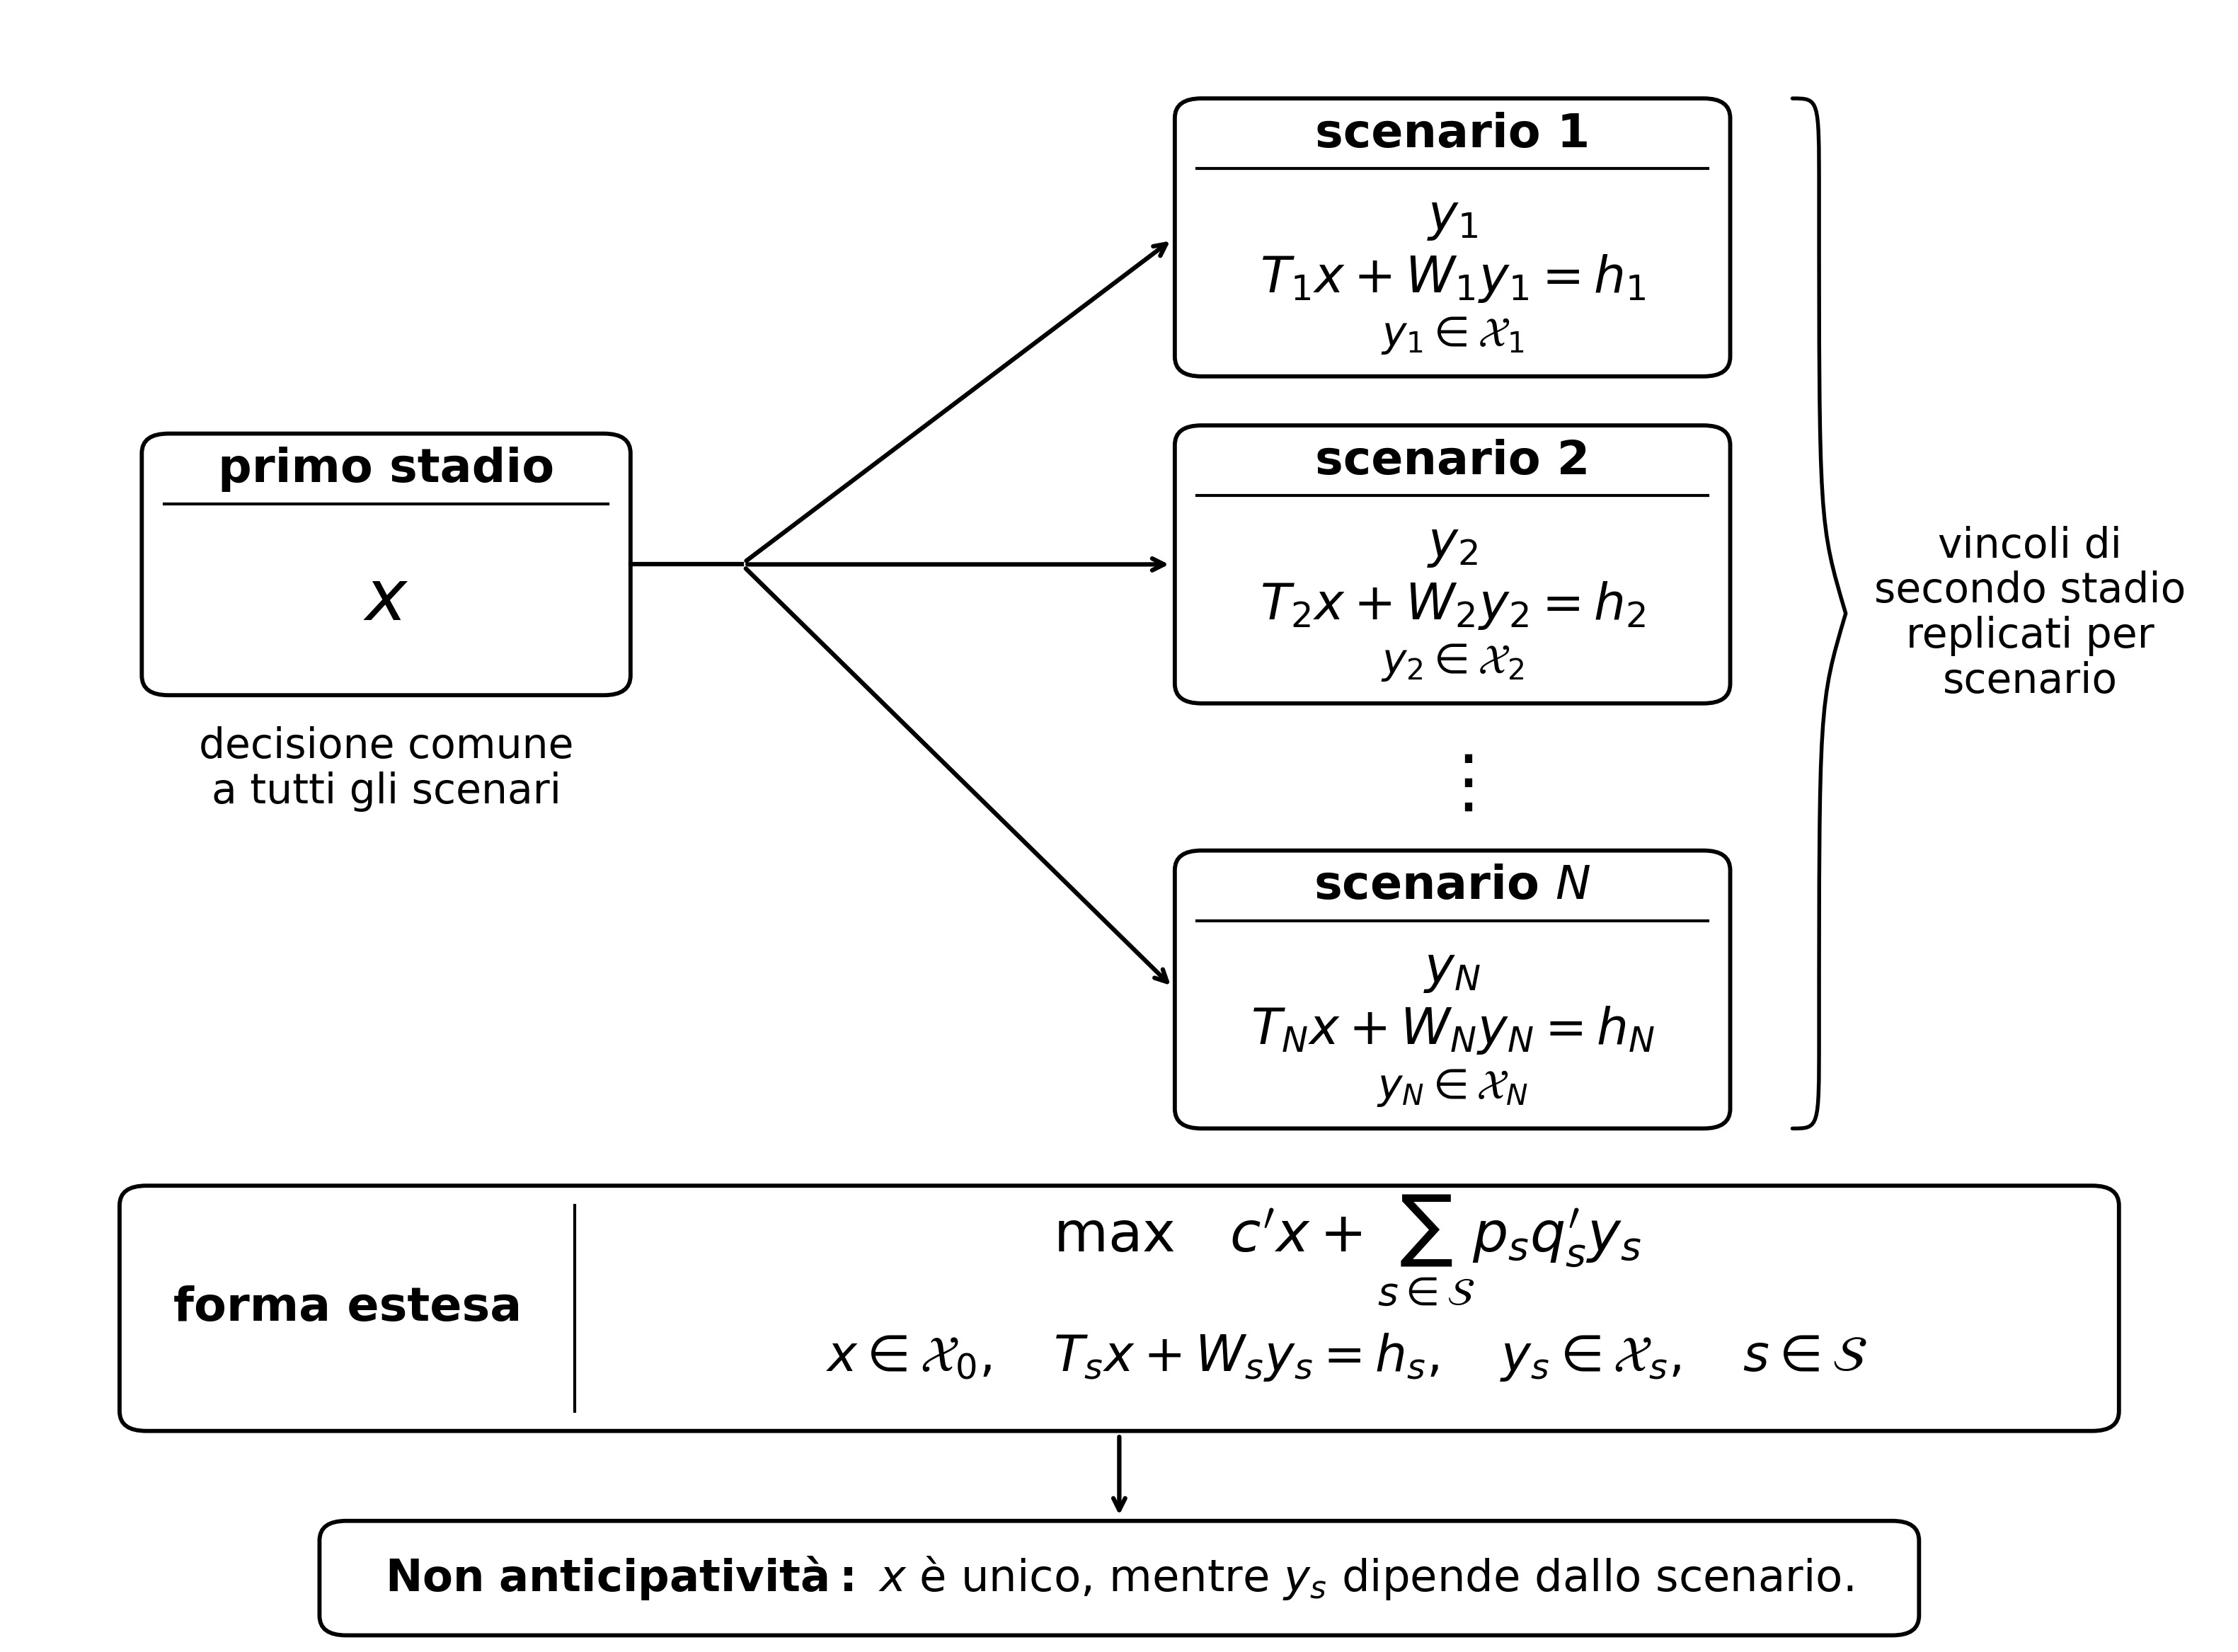
\includegraphics[width=0.55\textwidth]
{../graphics/Cap14_forma_estesa_blocchi.png}
\end{center}

\vspace{-2mm}

{\small $x$ compare in tutti i blocchi di scenario, ogni $y_s$ solo nei vincoli
del proprio scenario: \`e la struttura che la Lezione~16 passer\`a a
\texttt{linprog}.}

%TCIMACRO{\TeXButton{Transition: Box Out}{\transboxout}}%
%BeginExpansion
\transboxout%
%EndExpansion
%TCIMACRO{\TeXButton{EndFrame}{\end{frame}}}%
%BeginExpansion
\end{frame}%
%EndExpansion

%****************************************

\subsection{La consegna}%

%TCIMACRO{\TeXButton{BeginFrame}{\begin{frame}}}%
%BeginExpansion
\begin{frame}%
%EndExpansion

\QTR{frametitle}{Esercizio: forma estesa a tre scenari}

%TCIMACRO{\TeXButton{Transparency}{\setbeamercovered{transparent=20}}}%
%BeginExpansion
\setbeamercovered{transparent=20}%
%EndExpansion

{\footnotesize (Capitolo~14, Esercizio proposto~5)}

\medskip

{\small Tre scenari con $p_1=0.5$, $p_2=0.3$, $p_3=0.2$. Decisione di primo
stadio $x=(x_1,x_2)'$ con $x_1+x_2=12$, $x_1,x_2\geq0$; contributo
$c'x=1.2x_1+1.8x_2$. Ricorso $y_s=(g_s,u_s)'$ con $g_s,u_s\geq0$ e vincoli}
{\small
\[
x_1+0.9x_2+u_1-g_1=8,
\quad
x_1+0.6x_2+u_2-g_2=8,
\quad
x_1+0.3x_2+u_3-g_3=8.
\]
}
{\small Costi unitari del funding: $1$, $2$ e $5$.}

\medskip

\begin{stepenumerate}
\item [1.] Scrivere la forma estesa completa del problema.

\item [2.] Identificare le variabili di primo e di secondo stadio.

\item [3.] Scrivere la struttura matriciale a blocchi dei vincoli di secondo
stadio.

\item [4.] Spiegare perch\'e il vettore $x$ compare in tutti i blocchi mentre
ciascun $y_s$ compare in uno solo.
\end{stepenumerate}

%TCIMACRO{\TeXButton{Transition: Box Out}{\transboxout}}%
%BeginExpansion
\transboxout%
%EndExpansion
%TCIMACRO{\TeXButton{EndFrame}{\end{frame}}}%
%BeginExpansion
\end{frame}%
%EndExpansion

%****************************************

\subsection{La soluzione}%

%TCIMACRO{\TeXButton{BeginFrame}{\begin{frame}}}%
%BeginExpansion
\begin{frame}%
%EndExpansion

\QTR{frametitle}{Soluzione: un solo programma lineare}

%TCIMACRO{\TeXButton{Transparency}{\setbeamercovered{transparent=20}}}%
%BeginExpansion
\setbeamercovered{transparent=20}%
%EndExpansion

{\small
\[
\begin{array}{ll}
\max & 1.2x_1+1.8x_2-0.5u_1-0.6u_2-u_3\\[3pt]
\text{s.v.} & x_1+x_2=12,\\
& x_1+0.9x_2+u_1-g_1=8,\qquad x_1+0.6x_2+u_2-g_2=8,\\
& x_1+0.3x_2+u_3-g_3=8,\qquad x_1,x_2,g_s,u_s\geq0.
\end{array}
\]
}

{\small I coefficienti di $u_s$ sono probabilit\`a $\times$ costo:
$0.5\cdot1$, $0.3\cdot2$, $0.2\cdot5$. Otto variabili: $x=(x_1,x_2)'$ e
$y_s=(g_s,u_s)'$ per $s=1,2,3$.}

{\small
\[
\left(
\begin{array}{cc|cc|cc|cc}
1&0.9&-1&1&0&0&0&0\\
1&0.6&0&0&-1&1&0&0\\
1&0.3&0&0&0&0&-1&1
\end{array}
\right)
\begin{pmatrix}
x\\y_1\\y_2\\y_3
\end{pmatrix}
=
\begin{pmatrix}
8\\8\\8
\end{pmatrix}
\]
}

\begin{center}
{\small $x$ \`e unica perch\'e viene scelta prima dello scenario; ogni $y_s$
risponde a un solo scenario.}
\end{center}

%TCIMACRO{\TeXButton{Transition: Box Out}{\transboxout}}%
%BeginExpansion
\transboxout%
%EndExpansion
%TCIMACRO{\TeXButton{EndFrame}{\end{frame}}}%
%BeginExpansion
\end{frame}%
%EndExpansion

%****************************************

\section{Esercizio in aula: probabilit\`a di scenari da una catena di Markov}

\subsection{La consegna}%

%TCIMACRO{\TeXButton{BeginFrame}{\begin{frame}}}%
%BeginExpansion
\begin{frame}%
%EndExpansion

\QTR{frametitle}{Esercizio: probabilit\`a di scenari generati da una catena di Markov}

%TCIMACRO{\TeXButton{Transparency}{\setbeamercovered{transparent=20}}}%
%BeginExpansion
\setbeamercovered{transparent=20}%
%EndExpansion

{\footnotesize (Capitolo~14, Esercizio proposto~1)}

\medskip

Catena di Markov con stati $\mathcal I=\{z_1,z_2,z_3\}$, stato iniziale
$Z_0=z_2$, orizzonte di tre periodi e matrice di transizione
{\small
\[
P=
\begin{pmatrix}
0.5 & 0.3 & 0.2\\
0.2 & 0.6 & 0.2\\
0.1 & 0.4 & 0.5
\end{pmatrix}.
\]
}

\begin{stepenumerate}
\item [1.] Calcolare la probabilit\`a dello scenario $\xi_s=(z_1,z_2,z_3)$.

\item [2.] Calcolare la probabilit\`a dello scenario
$\xi_{s'}=(z_3,z_3,z_2)$.

\item [3.] Determinare $\Prob(Z_3=z_3\mid Z_0=z_2)$ utilizzando la matrice
$P^3$.

\item [4.] Spiegare perch\'e la probabilit\`a ottenuta al punto precedente non
coincide, in generale, con la probabilit\`a di uno specifico scenario che
termina in $z_3$.
\end{stepenumerate}

%TCIMACRO{\TeXButton{Transition: Box Out}{\transboxout}}%
%BeginExpansion
\transboxout%
%EndExpansion
%TCIMACRO{\TeXButton{EndFrame}{\end{frame}}}%
%BeginExpansion
\end{frame}%
%EndExpansion

%****************************************

\subsection{La soluzione}%

%TCIMACRO{\TeXButton{BeginFrame}{\begin{frame}}}%
%BeginExpansion
\begin{frame}%
%EndExpansion

\QTR{frametitle}{Soluzione: da dove vengono le $p_s$}

%TCIMACRO{\TeXButton{Transparency}{\setbeamercovered{transparent=20}}}%
%BeginExpansion
\setbeamercovered{transparent=20}%
%EndExpansion

\begin{stepenumerate}
\item [1.] $p_s=p_{21}\,p_{12}\,p_{23}=0.2\cdot0.3\cdot0.2=0.012$.

\item [2.] $p_{s'}=p_{23}\,p_{33}\,p_{32}=0.2\cdot0.5\cdot0.4=0.040$.

\item [3.] La riga di $z_2$ in $P^3$ si ottiene con
$\pi_{t+1}=\pi_tP$ da $\pi_0=(0,1,0)$:
{\small
\[
\pi_1=(0.2,\;0.6,\;0.2),
\qquad
\pi_2=(0.24,\;0.50,\;0.26),
\]
\[
\Prob(Z_3=z_3\mid Z_0=z_2)=0.24\cdot0.2+0.50\cdot0.2+0.26\cdot0.5=0.278.
\]
}

\item [4.] $0.278$ somma le probabilit\`a di \textbf{tutte} le traiettorie che
terminano in $z_3$; uno scenario \`e una sola di esse.
\end{stepenumerate}

\medskip

\begin{center}
{\small Gli scenari e le loro probabilit\`a $p_s$ sono i pesi della forma
estesa. Nel caso SVB-ALM vengono dalla catena a otto stati del
Capitolo~14.}
\end{center}

%TCIMACRO{\TeXButton{Transition: Box Out}{\transboxout}}%
%BeginExpansion
\transboxout%
%EndExpansion
%TCIMACRO{\TeXButton{EndFrame}{\end{frame}}}%
%BeginExpansion
\end{frame}%
%EndExpansion

%****************************************

\section{Vantaggi, limiti e sintesi}

\subsection{Vantaggi e limiti}%

%TCIMACRO{\TeXButton{BeginFrame}{\begin{frame}}}%
%BeginExpansion
\begin{frame}%
%EndExpansion

\QTR{frametitle}{Vantaggi e limiti della programmazione stocastica}

%TCIMACRO{\TeXButton{Transparency}{\setbeamercovered{transparent=20}}}%
%BeginExpansion
\setbeamercovered{transparent=20}%
%EndExpansion

\textbf{Vantaggi}
\begin{stepitemize}
\item Considera congiuntamente gli scenari, le loro probabilit\`a e le
possibilit\`a di ricorso.

\item Nel caso lineare la forma estesa si risolve con i metodi consolidati della
programmazione lineare, anche con vincoli finanziari e operativi articolati.
\end{stepitemize}

\medskip

\textbf{Costi}
\begin{stepitemize}
\item La qualit\`a della soluzione dipende dalla \textbf{rappresentativit\`a}
degli scenari e dall'\textbf{attendibilit\`a} delle probabilit\`a assegnate.

\item La dimensione cresce con il numero degli scenari: con $n_x$ variabili di
primo stadio e $n_y$ di ricorso per scenario, la forma estesa ha
$n_x+|\mathcal S|\,n_y$ variabili.
\end{stepitemize}

%TCIMACRO{\TeXButton{Transition: Box Out}{\transboxout}}%
%BeginExpansion
\transboxout%
%EndExpansion
%TCIMACRO{\TeXButton{EndFrame}{\end{frame}}}%
%BeginExpansion
\end{frame}%
%EndExpansion

%****************************************

\subsection{Programmazione robusta}%

%TCIMACRO{\TeXButton{BeginFrame}{\begin{frame}}}%
%BeginExpansion
\begin{frame}%
%EndExpansion

\QTR{frametitle}{Un approccio alternativo: la programmazione robusta}

%TCIMACRO{\TeXButton{Transparency}{\setbeamercovered{transparent=20}}}%
%BeginExpansion
\setbeamercovered{transparent=20}%
%EndExpansion

La programmazione robusta sostituisce alla distribuzione probabilistica un
insieme $\mathcal U$ di possibili realizzazioni dell'incertezza:
\[
\max_{x\in\mathcal X_0}
\left\{
c'x+
\inf_{\xi\in\mathcal U}Q(x,\xi)
\right\}.
\]

\begin{stepitemize}
\item Anzich\'e il risultato atteso, si massimizza il risultato
\textbf{garantito} nella realizzazione pi\`u sfavorevole dell'insieme.

\item Minore dipendenza da una distribuzione specificata; come contropartita,
decisioni pi\`u conservative.

\item La scelta dell'approccio dipende dalle informazioni probabilistiche
disponibili, dalla rilevanza degli scenari sfavorevoli e dalle risorse
computazionali.
\end{stepitemize}

%TCIMACRO{\TeXButton{Transition: Box Out}{\transboxout}}%
%BeginExpansion
\transboxout%
%EndExpansion
%TCIMACRO{\TeXButton{EndFrame}{\end{frame}}}%
%BeginExpansion
\end{frame}%
%EndExpansion

%****************************************

\subsection{Sintesi}%

%TCIMACRO{\TeXButton{BeginFrame}{\begin{frame}}}%
%BeginExpansion
\begin{frame}%
%EndExpansion

\QTR{frametitle}{Che cosa portiamo a casa}

%TCIMACRO{\TeXButton{Transparency}{\setbeamercovered{transparent=20}}}%
%BeginExpansion
\setbeamercovered{transparent=20}%
%EndExpansion

\begin{stepenumerate}
\item [1.] La \textbf{fattibilit\`a del ricorso} \`e il primo filtro: una
decisione iniziale attraente ma incompatibile con i limiti di funding non \`e
utilizzabile.

\item [2.] $Q_s(x)$ \`e \textbf{concava e lineare a tratti}: la decisione
iniziale cambia il problema che il secondo stadio dovr\`a risolvere.

\item [3.] La scelta di $x$ \`e un \textbf{compromesso} fra rendimento
iniziale e costo atteso del ricorso.

\item [4.] $\EVPI$ misura il valore dell'\textbf{informazione}, $\VSS$ quello
del \textbf{metodo}; $z^{EV}$ si calcola rivalutando $x^{EV}$ negli scenari.

\item [5.] La \textbf{forma estesa} \`e il programma lineare che il solver
riceve.
\end{stepenumerate}

\medskip

\begin{center}
{\small \textbf{Lezione~16}: SP, EV e WS calcolati in Python sul caso
SVB-ALM.}
\end{center}

%TCIMACRO{\TeXButton{Transition: Box Out}{\transboxout}}%
%BeginExpansion
\transboxout%
%EndExpansion
%TCIMACRO{\TeXButton{EndFrame}{\end{frame}}}%
%BeginExpansion
\end{frame}%
%EndExpansion

%****************************************

\end{document}
